%%%%%%%%%%%%%%%%%%%%%%%%%%%%%%%%%%%%%%%%%
% ELEE	3720 Electromechanical Energy Conversion: Report template
% By Ratheesh Ravindran
%%%%%%%%%%%%%%%%%%%%%%%%%%%%%%%%%%%%%%%%%
\documentclass[12pt]{article}
\usepackage[top=1in, bottom=1in, left=1in, right=1in]{geometry}
\usepackage[utf8x]{inputenc}
\usepackage{amsmath}
\usepackage{graphicx}
\graphicspath{{Images/}}
\usepackage[hidelinks]{hyperref}
\usepackage{multicol}
\usepackage{enumitem}
\usepackage{fancyhdr}
\usepackage{listings}
\usepackage{xcolor}
\usepackage{chngcntr}
\usepackage{caption}
\counterwithin{figure}{section}
\usepackage{framed,color,verbatim}
\definecolor{shadecolor}{rgb}{.9, .9, .9}

\newenvironment{block}%
   {\snugshade\verbatim}%
   {\endverbatim\endsnugshade}

\definecolor{codegreen}{rgb}{0,0.6,0}
\definecolor{codegray}{rgb}{0,0,0.5}
\definecolor{codepurple}{rgb}{0.58,0,0.82}
\definecolor{backcolour}{rgb}{0.95,0.95,0.92}
 
\lstdefinestyle{mystyle}{
    backgroundcolor=\color{backcolour},   
    commentstyle=\color{codegray},
    %keywordstyle=\color{magenta},
    numberstyle=\tiny\color{black},
    stringstyle=\color{codepurple},
    basicstyle=\ttfamily\footnotesize,
    breakatwhitespace=false,         
    breaklines=true,                 
    captionpos=b,                    
    keepspaces=true,                 
    numbers=left,                    
    numbersep=5pt,                  
    showspaces=false,                
    showstringspaces=false,
    showtabs=false,                  
    tabsize=2
}
 
\lstset{style=mystyle}
%\usepackage{fancyhdr}
%\pagestyle{fancy}
\begin{document}
\begin{titlepage}
\newcommand{\HRule}{\rule{\linewidth}{0.1mm}} 
\center % Center everything on the page
 
%---------------------------------------------------------------------------------
%	HEADING SECTIONS (Enter the Homework/assignment No., only)
%---------------------------------------------------------------------------------
%\textsc{\Large ELEE	3720}\\[0.5cm] % heading course Number
\textsc{\large STAT 5814: APPLIED TIME SERIES ANALYSIS}\\[0.5cm] % heading course name
%\textsc{\large Homework/Assignment No:- }\\[0.5cm] % Minor heading
%---------------------------------------------------------------------------------
%	TITLE SECTION (Replace 'TITLE' with the Homework/assignment Name/title)
%---------------------------------------------------------------------------------

\HRule \\[0.4cm]
{ \huge \textbf{Midterm Exam 2 Report}} % Title of your Homework/assignment
\HRule \\[1.5cm]
 
%---------------------------------------------------------------------------------
%	AUTHOR SECTION (EDIT THE NAME and T.NO., only)
%--------------------------------------------------------------------------------
\begin{multicols}{2}
\begin{minipage}[t]{0.45\textwidth}
\large
\emph{Submitted By:}\\
Sayantan Majumdar\\ \href{mailto:smxnv@mst.edu}{smxnv@mst.edu} \\
\end{minipage}
\begin{minipage}[t]{0.45\textwidth} \large
\begin{flushright}
\emph{Course Instructor:} \\
Dr. Akim Adekpedjou\\ \href{mailto: akima@mst.edu}{akima@mst.edu}\\ % Supervisor's Name
\end{flushright}
\end{minipage}
\end{multicols}
{\large \today}\\[1cm] % Date, change the \today to a set date if you want to be precise
\vspace{5pt}

\includegraphics[scale=0.3]{mst_logo_new.png}% \\[0.5cm] % 
\vfill % Fill the rest of the page with white-space

\end{titlepage}
%%
% GradingRubric.tex
% This page will be the 2nd page of your report and will be used for grading the homework/assignment.
\section*{Grading Rubric - Information to Students}

Grading rubric that will broadly apply to assessing performance. That is, assessment exercises that are associated with a predominantly qualitative rather than quantitative character. If, for a particular exercise, there is substantial deviation from the scheme outlined below, I will let you know! Note: Be aware that if your “Quality of Presentation” is poor, it could impact scores assigned for the other two categories! (DO NOT EDIT THIS PAGE)
%\hspace*{-1.5in}
\begin{figure}[ht!]
    \centering
    \includegraphics[scale=0.450]{LevelOfAccomplishments.png}
    \caption{Level of accomplishments}
    \label{fig:Level of accomplishments}
\end{figure}
\begin{table}[h]
    \centering
    \begin{tabular}{|c|c|}
    \hline
        Level &  Score \\
        \hline
        \hline
        5 &  12 (bonus!) \\
        \hline
        4: (`A`) &  10 \\
        \hline
        3: (`B`) &  8 \\
        \hline
        2: (`C`) &  6 \\
        \hline
        1: (`D`) &  4 \\
        \hline
        0: (`F`) &  0-2 \\
        \hline
    \end{tabular}
    \caption{Mapping of “Level” to “Score”}
    \label{tab:Mapping}
\end{table}
\begin{itemize}
    \item \textbf{Student's Level/Score (To be entered by Professor/GTA):}
\end{itemize}



\pagestyle{fancy}
\fancyhf{}
\chead{\small{\textit{STAT 5814 $\lvert$ Applied Time Series Analysis $\lvert$ Midterm Exam 2 $\lvert$ Sayantan Majumdar}}}
\rfoot{\thepage}
\renewcommand{\headheight}{26pt}
\tableofcontents          % Required
\listoffigures
%\listoftables
\newpage

% Do not edit the below sections, enter all details in respective chapters
% Add the images/screen-shorts to the image folder and insert them in the respective chapters
\section{Problem 1}
%\addcontentsline{toc}{section}{Problem 1}
%
% Abstract.tex

The monthly values of the average hourly for US apparel and textile workers for July 1981 to July 1987 are the file wages of the library TSA. 
\begin{enumerate}[label=(\alph*)]
    \item Plot the series and write a few lines on what you observe.
    \item Fit a linear trend model using least squares. Give the plot of the linear trend and superpose
it with that of the data. Give the estimated regression equation.
    \item Plot the standardized residuals from the linear regression versus time. Comments?
    \item Fit a quadratic time trend model using least squares. Give the plot of quadratic trend and
superpose it Give the estimated regression equation. Plot the residuals and comment on any patterns.
    \item Perform a diagnostic check of the residuals. Comments.
    \item Plot the autocorrelation function for the standardized residuals from the quadratic regression.
    \item Investigate the normality of the standardized residuals from the quadratic regression. Comment.
\end{enumerate}
\subsection{R Code}
\lstinputlisting[language=R]{Codes/Midterm_2_P1.R}
\subsection{Results}
\begin{enumerate}[label=(\alph*)]
    \item \begin{minipage}[!h]{\linewidth}
        \centering
        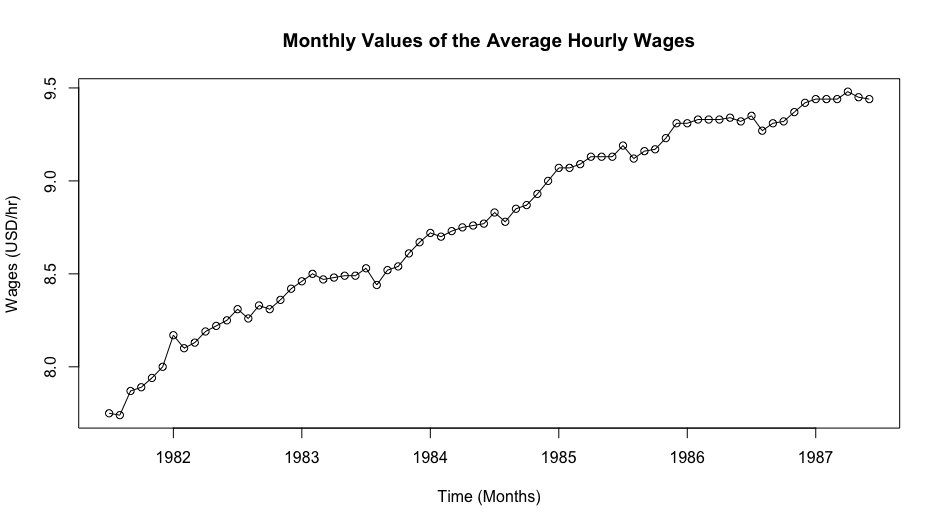
\includegraphics[width=\linewidth]{Images/P1/TS_Plot.png}
        \captionof{figure}[Time series plot of the wages data.]{Time series plot of the wages data. This shows that the wages are mostly increasing and only deviating from this trend in small proportions.}
        \label{fig:p1_ts}
    \end{minipage}
    \item Linear trend model fit summary: \small\begin{block}
Call:
lm(formula = wages ~ time(wages))

Residuals:
     Min       1Q   Median       3Q      Max 
-0.23828 -0.04981  0.01942  0.05845  0.13136 

Coefficients:
              Estimate Std. Error t value Pr(>|t|)    
(Intercept) -5.490e+02  1.115e+01  -49.24   <2e-16 ***
time(wages)  2.811e-01  5.618e-03   50.03   <2e-16 ***
---
Signif. codes:  0 ‘***’ 0.001 ‘**’ 0.01 ‘*’ 0.05 ‘.’ 0.1 ‘ ’ 1

Residual standard error: 0.08257 on 70 degrees of freedom
Multiple R-squared:  0.9728,	Adjusted R-squared:  0.9724 
F-statistic:  2503 on 1 and 70 DF,  p-value: < 2.2e-16
\end{block}
\normalsize
The R\textsuperscript{2} value of this fit is very good ($\approx 0.97$) which signifies that the linear fit is working well. The estimated regression equation is given by Eq \eqref{eq:reg}.
    \begin{equation}
    \label{eq:reg}
        \widehat{X_t} = -549 + 0.2811X_t + \varepsilon
    \end{equation}
    where $\varepsilon \sim \mathcal{N}(0, 0.08257)$ 
    \begin{figure}[!htb]
        \centering
        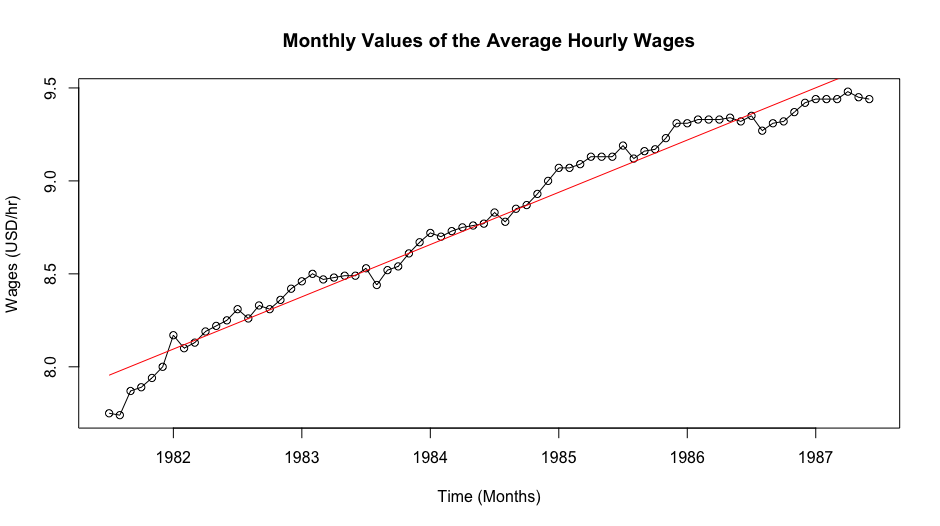
\includegraphics[width=0.9\linewidth]{Images/P1/Linear_Fit.png}
        \caption{Wages plot showing the linear trend in red.}
        \label{fig:lfit}
    \end{figure}
\item 
    \begin{minipage}[!h]{\linewidth}
        \centering
        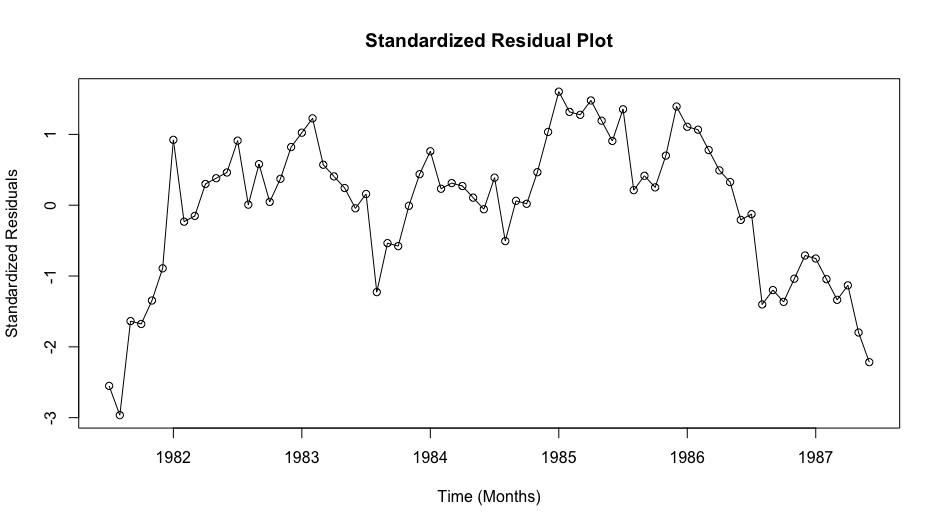
\includegraphics[width=0.9\linewidth]{Images/P1/SR_Plot.png}
        \captionof{figure}[Standardized residuals from the linear regression versus time.]{Standardized residuals from the linear regression versus time. Since the majority of the standardized residuals are within the [-2, 1] interval, so the model residuals strongly follow a normal distribution. Hence, we have a good fit.}
            \label{fig:sr}
    \end{minipage}
\item Quadratic time trend model summary: \small\begin{block}
Call:
lm(formula = wages ~ time(wages) + I(time(wages)^2))

Residuals:
      Min        1Q    Median        3Q       Max 
-0.148318 -0.041440  0.001563  0.050089  0.139839 

Coefficients:
                   Estimate Std. Error t value Pr(>|t|)    
(Intercept)      -8.495e+04  1.019e+04  -8.336 4.87e-12 ***
time(wages)       8.534e+01  1.027e+01   8.309 5.44e-12 ***
I(time(wages)^2) -2.143e-02  2.588e-03  -8.282 6.10e-12 ***
---
Signif. codes:  0 ‘***’ 0.001 ‘**’ 0.01 ‘*’ 0.05 ‘.’ 0.1 ‘ ’ 1

Residual standard error: 0.05889 on 69 degrees of freedom
Multiple R-squared:  0.9864,	Adjusted R-squared:  0.986 
F-statistic:  2494 on 2 and 69 DF,  p-value: < 2.2e-16
\end{block}  
\normalsize
The R\textsuperscript{2} value of this fit is even better ($\approx 0.98$) when compared to the linear fit earlier. This implies that the quadratic trend is more appropriate. The estimated regression equation is given by Eq \eqref{eq:regq}.
    \begin{equation}
    \label{eq:regq}
        \widehat{X_t} = -84950 + 85.34X_t - 0.02143X^2_t + \varepsilon
    \end{equation}
    where $\varepsilon \sim \mathcal{N}(0, 0.05889)$ 
    \begin{figure}[!h]
        \centering
        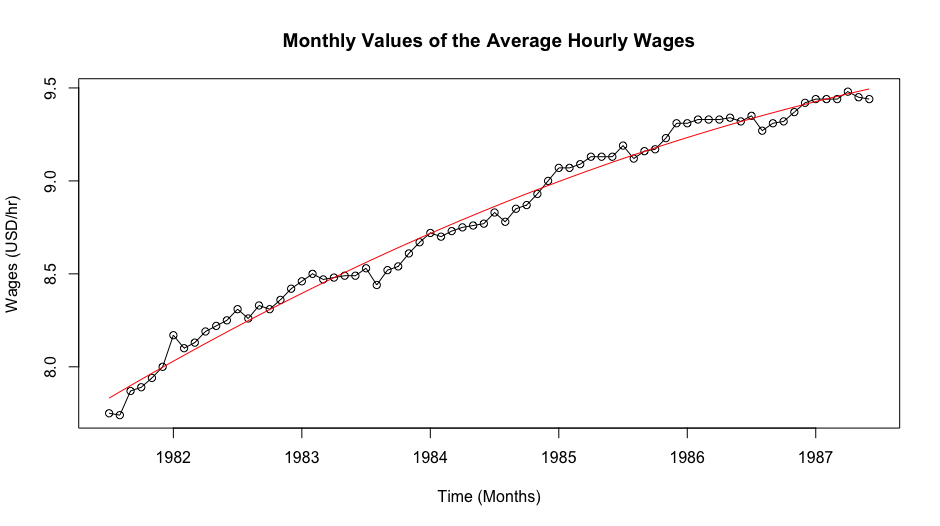
\includegraphics[width=0.9\linewidth]{Images/P1/Q_Fit.png}
        \caption{Wages plot showing the quadratic fit in red.}
        \label{fig:qfit}
    \end{figure}
    \begin{figure}[!h]
        \centering
        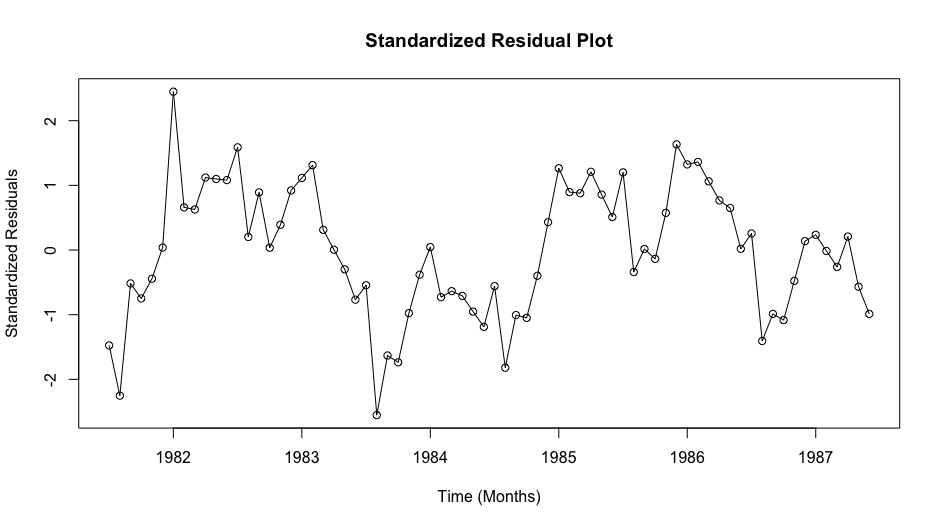
\includegraphics[width=0.9\linewidth]{Images/P1/SR_plot_q.png}
        \caption[Standardized residual plot for the quadratic fit.]{Standardized residual plot for the quadratic fit. Here, we observe that these most of these residuals are in the $\pm2$ region. So, the quadratic fit is better than the linear one.}
        \label{fig:sr_q}
    \end{figure}
\item 
\begin{minipage}[!h]{\linewidth}
    \centering
    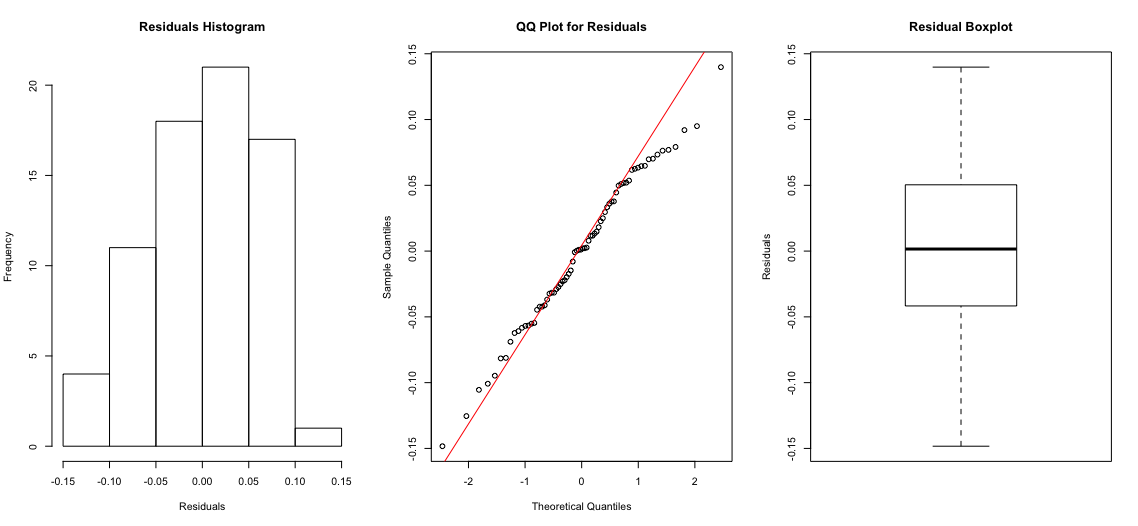
\includegraphics[width=\linewidth]{Images/P1/RD_P1.png}
    \captionof{figure}[Residual diagnostics of the quadratic model.]{Residual diagnostics of the quadratic model showing residual histogram, qq-plot, and boxplot. These plots show that the residuals closely follow a normal distribution.}
    \label{fig:rd_p1}
\end{minipage}
\item \begin{minipage}[!h]{\linewidth}
\centering
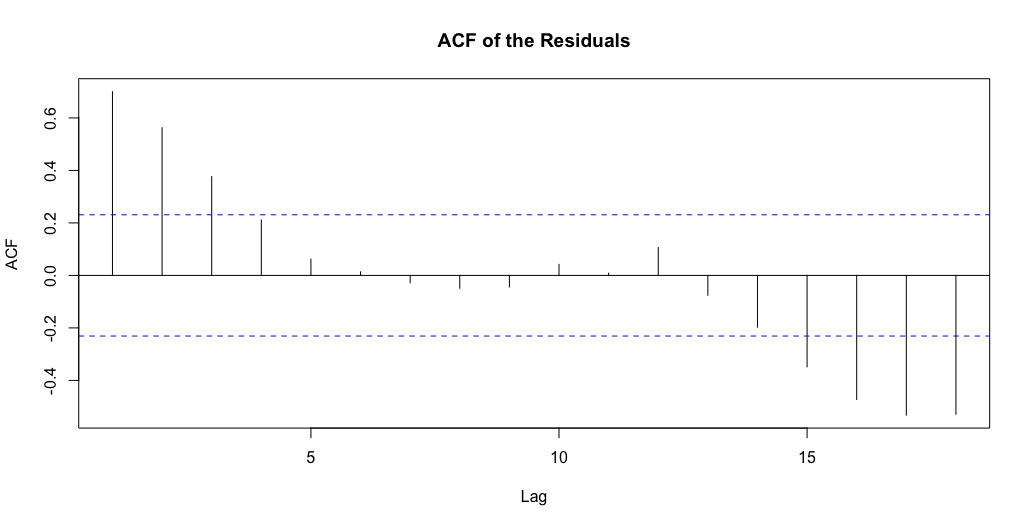
\includegraphics[width=0.9\linewidth]{Images/P1/ACF_P1.png}
\captionof{figure}[Autocorrelation  function (ACF)  for  the  standardized  residuals  from  the  quadratic regression.]{Autocorrelation  function (ACF)  for  the  standardized  residuals  from  the  quadratic regression. This shows that the ACF quickly degrades to zero as the lag increases.}
\end{minipage}
\item Residual normality checks: \small\begin{block}
Shapiro-Wilk normality test
data:  wages.qm$residuals
W = 0.98856, p-value = 0.7622

Exact runs test
data:  wages.qm$residuals
Runs = 15, p-value = 1.284e-07
alternative hypothesis: two.sided
\end{block}
\normalsize
The Shapiro-Wilk test shows that the residuals are normally distributed (p-value $>$ 0.05 and W is close to 1). However, the runs test suggests that the order of the residuals is not random. 
\end{enumerate}

\section{Problem 2}
%\addcontentsline{toc}{section}{Problem 2}
A data set of 57 consecutive measurements from a machine tool are in the TSA package.
\begin{enumerate}[label=(\alph*)]
    \item Estimate the parameters of a (mean-centered) AR(1) model for this series. Use the least
squares method and maximum likelihood, and report the estimated parameters from each of
these methods. Comment on any similarities and differences. Give the confidence intervals of
your parameters.
    \item Estimate the parameters of a (mean-centered) AR(2) model for this series. Use the least
squares method and maximum likelihood, and report the estimated parameters from each of
these methods. Comment on any similarities and differences.
    \item Derive the confidence intervals for the parameters $\phi_1$ and $\phi_2$. Does the confidence interval for $\phi_2$ suggests it should be included in the model?
    \item Compare the results of the maximum likelihood fits from parts (a) and (b). Which model
do you believe is preferable? Briefly explain your answer.
    \item Perform a diagnostic check of the residuals. Comments.
    \item Compare the two models using AIC, BIC. Which one do you prefer? Does any of the
quantities suggests one model is better than the other? If so, how much do you gain in errors reduction if any. Is that in line with your answer in (d)?
\end{enumerate}

\subsection{R Code}
\lstinputlisting[language=R]{Codes/Midterm_2_P2.R}
\newpage
\subsection{Results}
\begin{figure}[!htb]
    \centering
    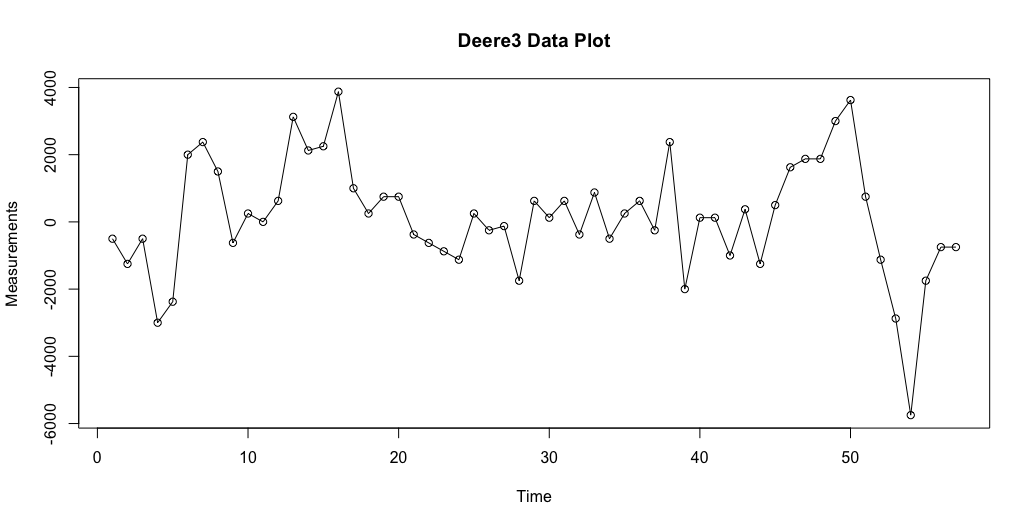
\includegraphics[width=0.9\linewidth]{Images/P2/TS_Plot_P2.png}
    \caption{Time series plot of the Deere3 data.}
    \label{fig:deere3}
\end{figure}
\begin{enumerate}[label=(\alph*)]
    \item Least squares method for AR(1) parameter estimation: \small\begin{block}
> print(css_model_ar1_coef)
        ar1   intercept 
  0.5332044 160.0797248 
> confint(css_model_ar1)
                 2.5 %      97.5 %
ar1          0.3132122   0.7531966
intercept -646.0111173 966.1705670
\end{block}
\normalsize Maximum Likelihood method for AR(1) parameter estimation: \small\begin{block}
> print(ml_model_ar1_coef)
        ar1   intercept 
  0.5255778 124.3524257 
> confint(ml_model_ar1)
                 2.5 %      97.5 %
ar1          0.3084104   0.7427452
intercept -648.3281895 897.0330409
\end{block}
\normalsize The estimated $\hat\phi$ from both the least squares and maximum likelihood methods are very similar. However, the intercept ($\hat\mu$) is significantly different. In addition, the confidence intervals for $\hat\phi$ in both cases are similar and $0 \not\in$ CI($\hat\phi$). 
    \item Least squares method for AR(2) parameter estimation: \small\begin{block}
> print(css_model_ar2_coef)
         ar1          ar2    intercept 
5.245848e-01 7.938728e-03 2.011876e+02 
\end{block}
\normalsize Maximum Likelihood method for AR(2) parameter estimation: \small\begin{block}
> print(ml_model_ar2_coef)
         ar1          ar2    intercept 
  0.52111096   0.00830321 123.24182209 
\end{block}
\normalsize Like before, the estimated $\phi_1$ and $\phi_2$ in both cases are pretty similar, whereas, the intercepts are significantly different. 
\item Confidence intervals for $\phi_1$ and $\phi_2$: \small\begin{block}
Least Squares Method
> confint(css_model_ar2)
                 2.5 %       97.5 %
ar1          0.2660503    0.7831192
ar2         -0.2509164    0.2667939
intercept -607.0745845 1009.4498459

Maximum Likelihood Method
> confint(ml_model_ar2)
                 2.5 %      97.5 %
ar1          0.2642641   0.7779579
ar2         -0.2493401   0.2659465
intercept -656.0388502 902.5224944
\end{block}
\normalsize Since $0 \in$ CI($\phi_2$), therefore, $\phi_2 \approx 0$. So $\phi_2$ should not be included in the model.
\item \label{answer_ref_d} The maximum likelihood estimates of the intercepts for the AR(1) and AR(2) models are pretty similar. Also, the confidence interval of the intercept in case of AR(1) is a subset of that of AR(2). But, since our target is develop a parsimonious model and $0 \in$ CI($\phi_2$) for the maximum likelihood method as well, so, AR(1) is the preferable model. 

\item Residual Diagnostics:
\begin{figure}[!htb]
    \centering
    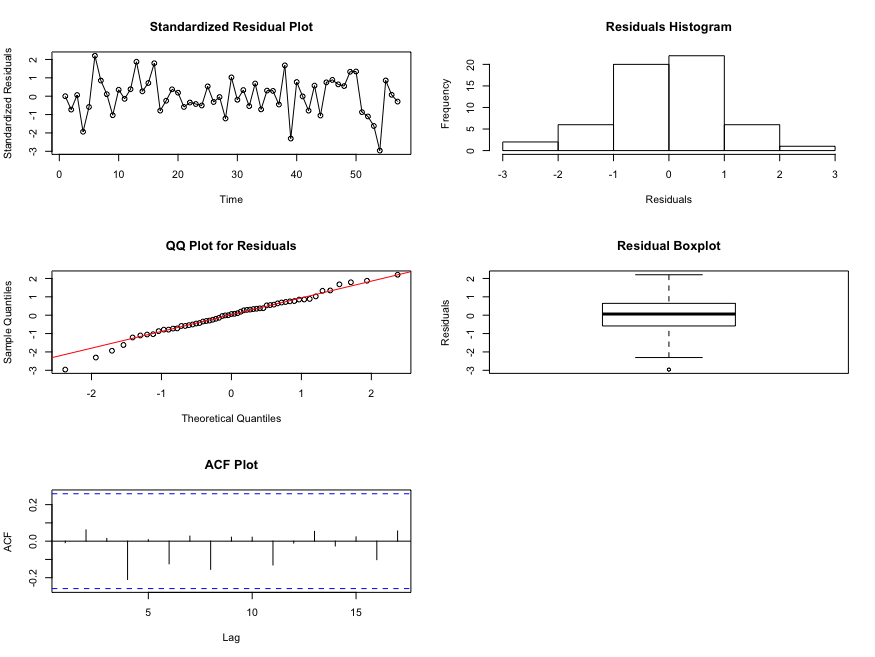
\includegraphics[width=\linewidth]{Images/P2/Residual_CSS_AR1.png}
    \caption[Residual diagnostic plots for least squares estimation for AR(1).]{Residual diagnostic plots for least squares estimation for AR(1). These plots shows that the residuals tend to closely follow a normal distribution.}
    \label{fig:residual_css_ar1}
\end{figure}
\begin{figure}[!htb]
    \centering
    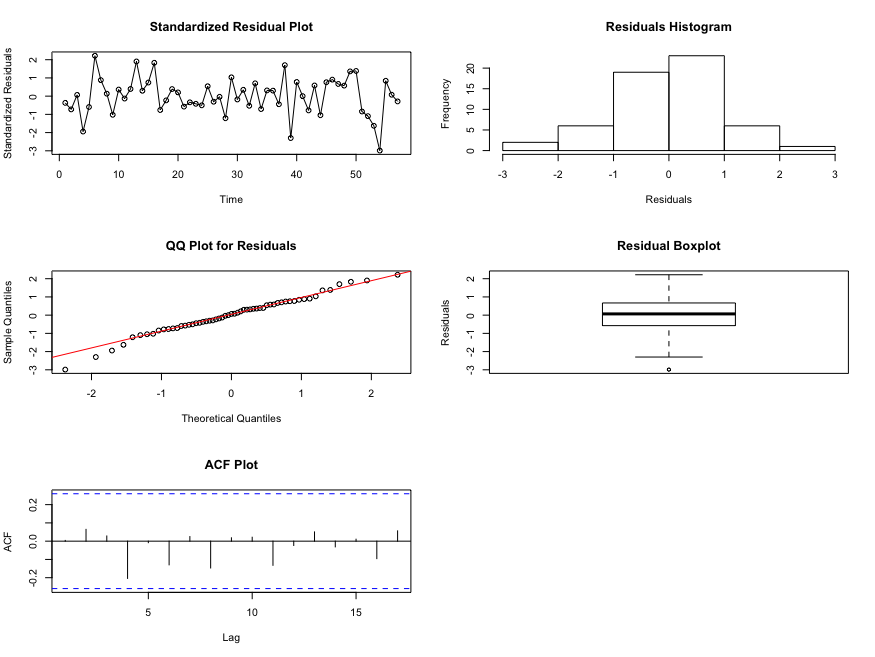
\includegraphics[width=\linewidth]{Images/P2/Residual_ML_AR1.png}
    \caption[Residual diagnostic plots for maximum likelihood estimation for AR(1)]{Residual diagnostic plots for maximum likelihood estimation for AR(1). Similar observations like that of Fig \ref{fig:residual_css_ar1} can be made.}
\end{figure}
\begin{figure}[!htb]
    \centering
    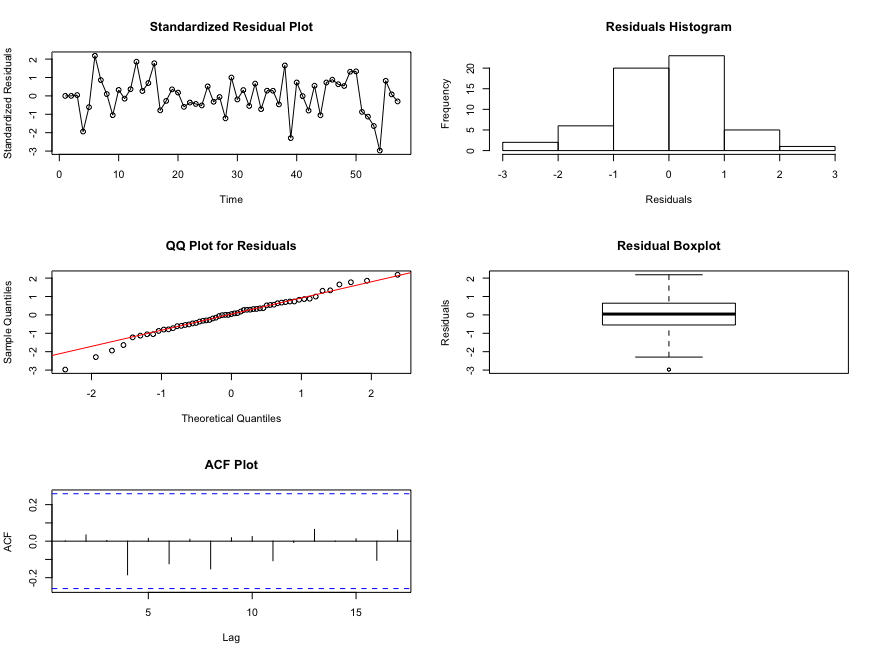
\includegraphics[width=\linewidth]{Images/P2/Residual_CSS_AR2.png}
    \caption[Residual diagnostic plots for least squares estimation for AR(2).]{Residual diagnostic plots for least squares estimation for AR(2). Like before, these also closely follow a normal distribution but less than AR(1) residuals.}
    \label{fig:residual_css_ar2}
\end{figure}
\begin{figure}[!htb]
    \centering
    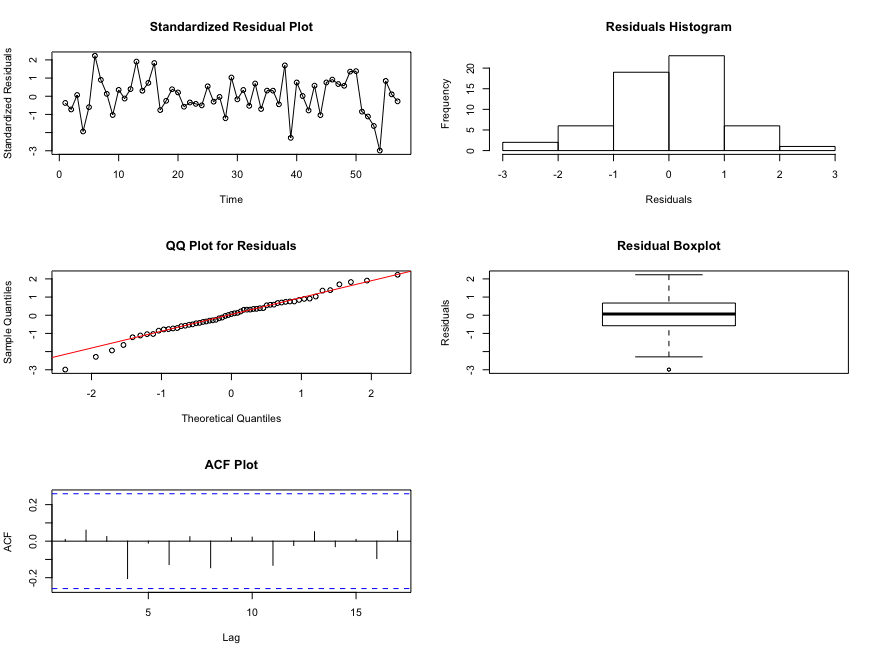
\includegraphics[width=\linewidth]{Images/P2/Residual_ML_AR2.png}
    \caption[Residual diagnostic plots for maximum likelihood estimation for AR(2).]{Residual diagnostic plots for maximum likelihood estimation for AR(2). Similar observations like that of Fig \ref{fig:residual_css_ar2} can be made.}
\end{figure}
The residual normality test results are given below. \small\begin{block}
Least Squares Estimation for AR(1):

Shapiro-Wilk normality test
data:  st_residuals
W = 0.98297, p-value = 0.6

Exact runs test
data:  st_residuals
Runs = 29, p-value = 1

Maximum Likelihood Estimation for AR(1):

Shapiro-Wilk normality test
data:  st_residuals
W = 0.98261, p-value = 0.5827

Exact runs test
data:  st_residuals
Runs = 29, p-value = 1

Least Squares Estimation for AR(2):

Shapiro-Wilk normality test
data:  st_residuals
W = 0.9809, p-value = 0.5028

Exact runs test
data:  st_residuals
Runs = 29, p-value = 1

Maximum Likelihood Estimation for AR(2):

Shapiro-Wilk normality test
data:  st_residuals
W = 0.98294, p-value = 0.599

Exact runs test
data:  st_residuals
Runs = 29, p-value = 1
\end{block}
\normalsize The normality tests show that the residuals from the AR(1) tend to follow the normal distribution more closely than those of AR(2).
\item AIC and BIC tests for the maximum likelihood method: \small\begin{block}
AR(1):
> AIC(model)
[1] 997.0189
> BIC(model)
[1] 1003.148

AR(2):
> AIC(model)
[1] 999.0148
> BIC(model)
[1] 1007.187
\end{block}
\normalsize As observed, we obtain a reduction of $\approx 2$ and $\approx 4$ in the AIC and BIC values respectively for the AR(1) model. Although, these are not significant reductions, our aim is always to develop a parsimonious model which aligns with the results obtained in \ref{answer_ref_d}. Therefore, AR(1) is the preferred model which is further confirmed using the auto.arima function in R.
\small\begin{block}
> auto_arima
Series: deere3 
ARIMA(1,0,0) with zero mean 

Coefficients:
         ar1
      0.5291
s.e.  0.1103

sigma^2 estimated as 2109761:  log likelihood=-495.56
AIC=995.12   AICc=995.34   BIC=999.2
\end{block}
\end{enumerate}

\section{Problem 3}
%\addcontentsline{toc}{section}{Problem 3}
Are sales trends for two industrial products related? The two time series objects described below contain Sales of chemicals and allied products; and Sales of motor vehicles and parts, in the U.S. for each month from Jan. 1971 to Dec. 1991. File is petr.txt. \\

\noindent You should analyze the data in the "chemicals" time series and the "vehicles" time series and write a report to address such questions as:
\begin{enumerate}[label=(\roman*)]
    \item What trend model(s) best capture the trends in sales of chemicals over time?
    \item What trend model(s) best capture the trends in sales of vehicles over time? Once the trend
has been accounted for, what can you say about the behavior of the detrended data, for both
models? Can either the original time series or the detrended series be described using any
common models?
    \item For the various models you tried, assess their fit. Can any transformations improve the
fit? Is there any apparent association between chemical sales and vehicle sales over time? If so,
describe the association.
    \item Make conclusions that relate to how the sales amounts (for both chemicals and vehicles)
change, both long-term over the observed period of years, and in terms of patterns of month-
to-month variation.
\end{enumerate}

\subsection{R Code}
\lstinputlisting[language=R]{Codes/Midterm_2_P3.R}
\subsection{Results}
\begin{enumerate}[label=(\roman*)]
    \item \begin{minipage}[!h]{0.9\linewidth}
    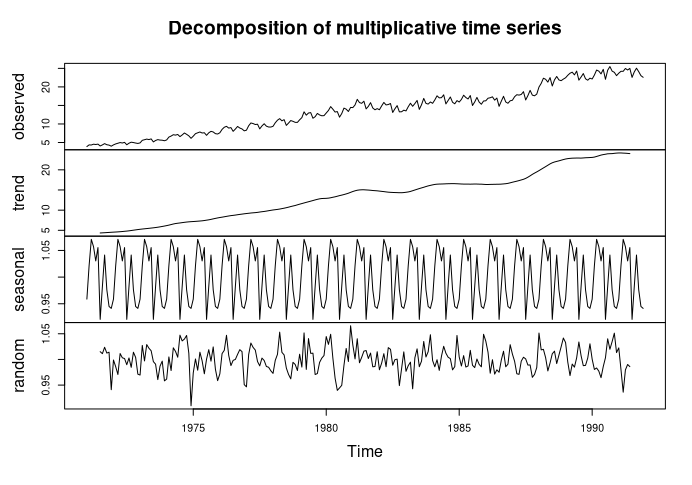
\includegraphics[width=\linewidth]{Images/P3/Chemicals_Plot.png}
    \captionof{figure}[Decomposition of the Chemicals data.]{Decomposition of the Chemicals data shows that both trend and seasonality are present.}
    \end{minipage}
    
    \item \begin{minipage}[!h]{0.9\linewidth}
    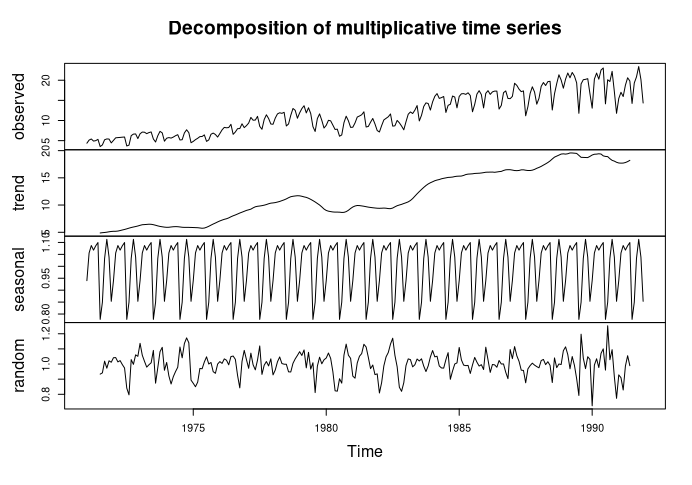
\includegraphics[width=\linewidth]{Images/P3/Vehicles_Plot.png}
    \captionof{figure}[Decomposition of the Vehicles data.]{Decomposition of the Vehicles data.}
    \end{minipage} \\
    Here, we again observe that the data exhibit both trend and seasonality. Nevertheless, in both the cases, we check their stationarity.
    \small\begin{block}
> adf.test(chemicals.data)

Augmented Dickey-Fuller Test
data:  chemicals.data
Dickey-Fuller = -3.0203, Lag order = 6, p-value = 0.1462
alternative hypothesis: stationary

> adf.test(vehicles.data)
Augmented Dickey-Fuller Test
data:  vehicles.data
Dickey-Fuller = -2.9112, Lag order = 6, p-value = 0.1921
alternative hypothesis: stationary
\end{block}
\normalsize The augmented Dickey-Fuller tests for both the datasets fail to reject the null hypothesis, and hence, these time series data are not stationary. Therefore, we detrend (also remove seasonality) these, and the time series plots are shown in Fig \ref{fig:diff_plots}.
\begin{figure}[!htb]
    \centering
    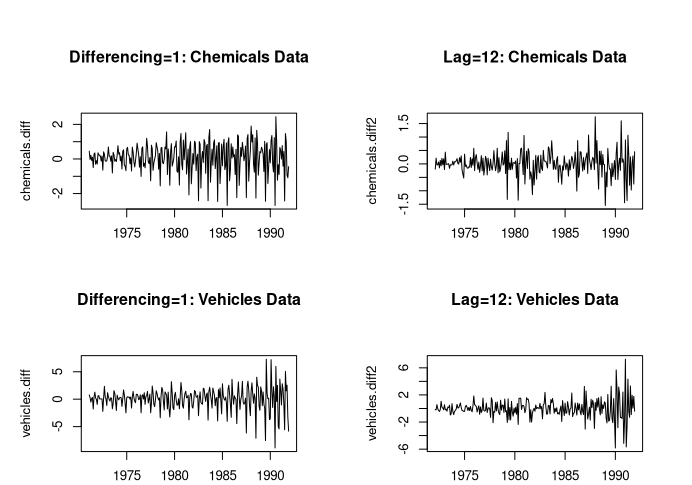
\includegraphics[width=\linewidth]{Images/P3/Diff_Plots.png}
    \caption[Time series plots of the detrended data.]{Time series plots of the detrended data. At first, the linear trend is removed using the first differences. Then the seasonality of the differenced data is removed by setting lag=12 as we deal with monthly data here.}
    \label{fig:diff_plots}
\end{figure}

The visual observation of the final detrended (Fig \ref{fig:diff_plots}) data show that both the time series have become stationary. We further test this using the augmented Dickey-Fuller test which confirms that we have achieved stationarity.
\small\begin{block}
> adf.test(chemicals.diff2)

Augmented Dickey-Fuller Test
data:  chemicals.diff2
Dickey-Fuller = -5.6096, Lag order = 6, p-value = 0.01
alternative hypothesis: stationary

> adf.test(vehicles.diff2)

Augmented Dickey-Fuller Test
data:  vehicles.diff2
Dickey-Fuller = -7.1672, Lag order = 6, p-value = 0.01
alternative hypothesis: stationary
\end{block}
\normalsize Here, the original data can be described as a harmonic model with increasing trend. However, for the detrended data, we can calculate the ACF, PACF, and EACF to get an idea about the order of the ARIMA process.  
\item Initally, we check the result of the harmonic model fit over the original data. \small\begin{block}
Call:
lm(formula = chemicals.data ~ har + time(chemicals.data))

Residuals:
    Min      1Q  Median      3Q     Max 
-4.0447 -0.5332  0.0430  0.6677  3.0799 

Coefficients:
                       Estimate Std. Error t value Pr(>|t|)    
(Intercept)          -1.951e+03  2.365e+01 -82.478  < 2e-16 ***
harcos(2*pi*t)       -9.564e-02  1.023e-01  -0.935    0.351    
harsin(2*pi*t)        5.420e-01  1.023e-01   5.297  2.6e-07 ***
time(chemicals.data)  9.913e-01  1.194e-02  83.058  < 2e-16 ***
---
Signif. codes:  0 ‘***’ 0.001 ‘**’ 0.01 ‘*’ 0.05 ‘.’ 0.1 ‘ ’ 1

Residual standard error: 1.148 on 248 degrees of freedom
Multiple R-squared:  0.9653,	Adjusted R-squared:  0.9649 
F-statistic:  2302 on 3 and 248 DF,  p-value: < 2.2e-16

Call:
lm(formula = vehicles.data ~ har + time(vehicles.data))

Residuals:
    Min      1Q  Median      3Q     Max 
-7.0874 -1.3989  0.3886  1.5226  4.5814 

Coefficients:
                      Estimate Std. Error t value Pr(>|t|)    
(Intercept)         -1.499e+03  4.476e+01 -33.497  < 2e-16 ***
harcos(2*pi*t)       2.120e-01  1.935e-01   1.095  0.27449    
harsin(2*pi*t)       5.378e-01  1.936e-01   2.777  0.00591 ** 
time(vehicles.data)  7.626e-01  2.259e-02  33.760  < 2e-16 ***
---
Signif. codes:  0 ‘***’ 0.001 ‘**’ 0.01 ‘*’ 0.05 ‘.’ 0.1 ‘ ’ 1

Residual standard error: 2.172 on 248 degrees of freedom
Multiple R-squared:  0.8217,	Adjusted R-squared:  0.8195 
F-statistic: 380.9 on 3 and 248 DF,  p-value: < 2.2e-16
\end{block}
\normalsize While the R\textsuperscript{2} is good for both cases, the residual standard error is quite high along with the F-statistic. The model fits for both the original datasets are depicted in Fig \ref{fig:harmonic_fit}. 
\begin{figure}[!htb]
    \centering
    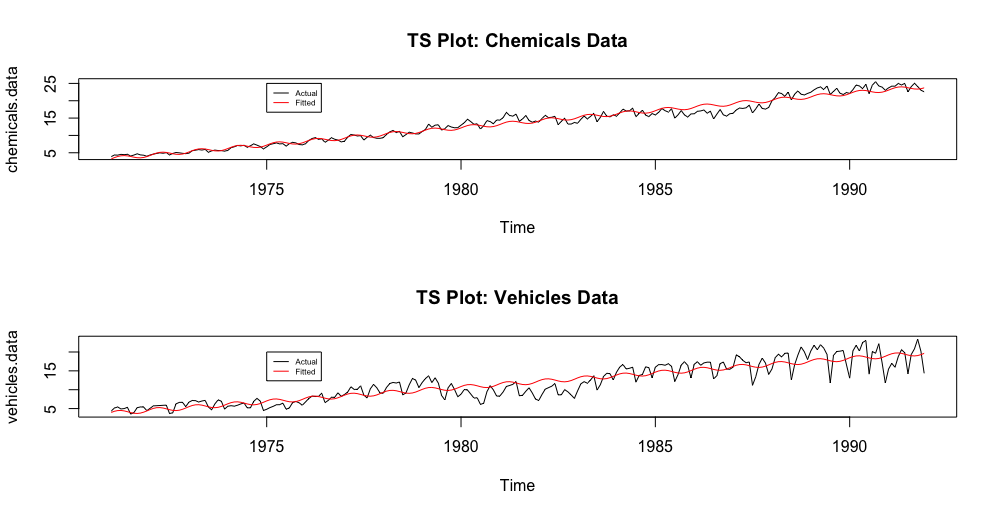
\includegraphics[width=\linewidth]{Images/P3/LFits_Original.png}
    \caption[Fitting a harmonic model with linear trend over the original data.]{Fitting a harmonic model with linear trend over the original data. We see that this model somewhat matches the time series pattern but misses out a lot. Increasing the number of harmonic pairs better fits the model but could lead to possible overfitting and results in a non-parsimonious model.}
    \label{fig:harmonic_fit}
\end{figure}
We now perform the residual diagnostics of the fit. 
\begin{figure}[!htb]
    \centering
    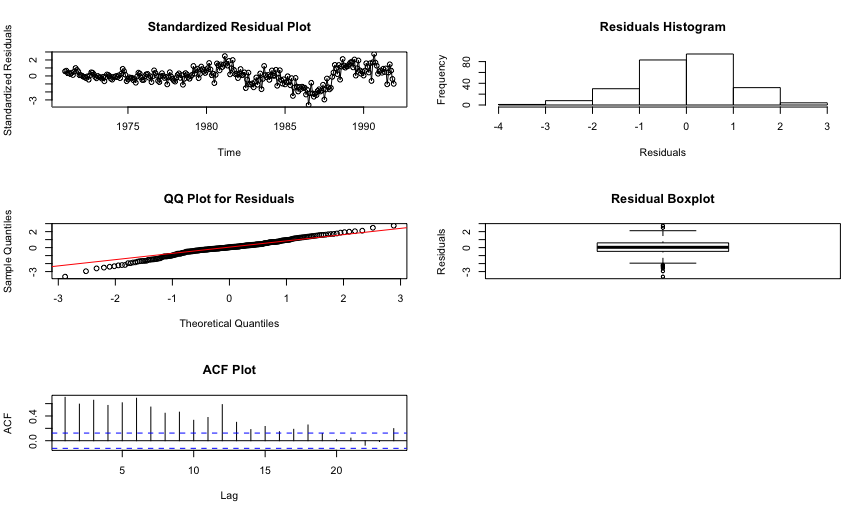
\includegraphics[width=\linewidth]{Images/P3/LFit_Res_Chem.png}
    \caption[Residual diagnostics of the harmonic fit over the original Chemicals data.]{Residual diagnostics of the harmonic fit over the original Chemicals data. Here, we see the non-normality of the residuals.}
    \label{fig:res_chem_har}
\end{figure}
\begin{figure}[!htb]
    \centering
    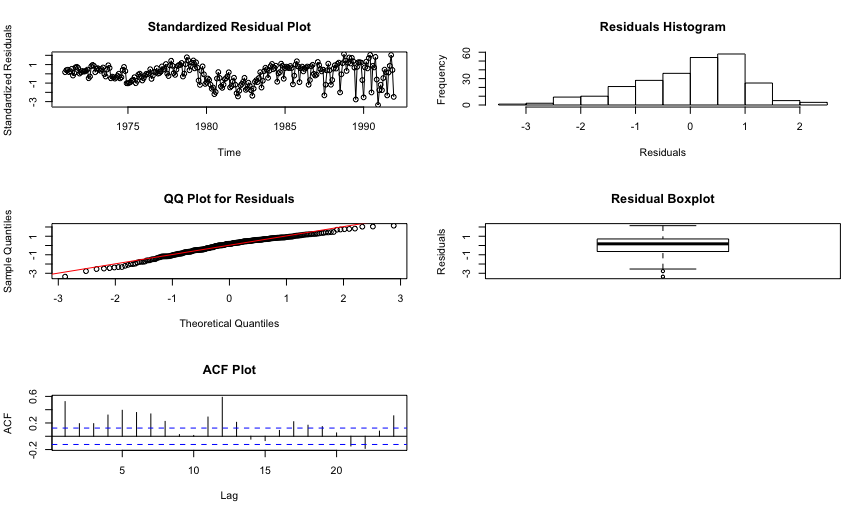
\includegraphics[width=\linewidth]{Images/P3/LFit_Res_Veh.png}
    \caption[Residual diagnostics of the harmonic fit over the original Vehicles data.]{Residual diagnostics of the harmonic fit over the original Vehicles data. Here, we again see the non-normality of the residuals.}
    \label{fig:res_veh_har}
\end{figure}
Furthermore, we check the AIC and BIC values along with the p-values of the normality checks. Both the normality checks suggest that the residuals are from a non-normal distribution. 
\small\begin{block}
Original Chemicals Data

Shapiro-Wilk normality test
W = 0.98358, p-value = 0.005282

Exact runs test
Runs = 56, p-value < 2.2e-16
alternative hypothesis: two.sided

> AIC(chemicals.fit)
[1] 790.5797
> BIC(chemicals.fit)
[1] 808.2269

Original Vehicles Data

Shapiro-Wilk normality test
W = 0.98358, p-value = 0.005282

Exact runs test
Runs = 56, p-value < 2.2e-16
alternative hypothesis: two.sided

> AIC(vehicles.fit)
[1] 1112.108
> BIC(vehicles.fit)
[1] 1129.755
\end{block}
\normalsize Now, we observe the ACF, PACF, EACF, and ARMA Subset Plots for the detrended data.
\begin{figure}[!htb]
    \centering
    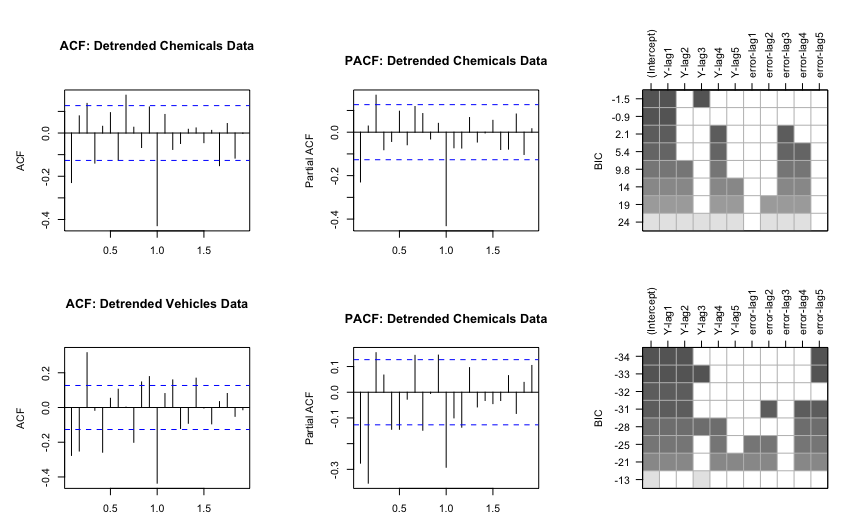
\includegraphics[width=\linewidth]{Images/P3/ACFs_Detrended.png}
    \caption[ACF, PACF, and ARMA subset plots for the detrended Chemicals and Vehicles data.]{ACF, PACF, and ARMA subset plots for the detrended Chemicals and Vehicles data. These show that the detrended data could possible have both AR and MA parts.}
    \label{fig:acf_det}
\end{figure}
The EACF matrices for these data are given below.
\small\begin{block}
> eacf(chemicals.diff2)
AR/MA
  0 1 2 3 4 5 6 7 8 9 10 11 12 13
0 x o x x o o o x o o o  x  o  o 
1 o o x o o o o x o o o  x  o  o 
2 x x o o o o o x o o o  x  o  x 
3 x x x o o o o o o o o  x  o  x 
4 x x o o o o o o o o o  x  o  x 
5 x x o o o o o o o o o  x  x  o 
6 x x o x x o o o o o o  x  o  o 
7 x x x x o o o o o o o  x  o  o 

> eacf(vehicles.diff2)
AR/MA
  0 1 2 3 4 5 6 7 8 9 10 11 12 13
0 x x x o x o o o x x x  x  o  x 
1 x x x o x o o o x o o  x  x  x 
2 x x o x x o o o o o o  x  o  x 
3 x x x o x o o o o o o  x  x  x 
4 x x o o o o o o o o o  x  x  x 
5 x x x o x o o o o o o  x  x  o 
6 x x o x x o o o o o o  x  x  o 
7 x x o o o o o o o o o  x  x  o 
\end{block}
\normalsize Next, we fit the best ARIMA model using the auto.arima function in R and perform the necessary residual diagnostics (using tsdiag function). These are shown in Figures \ref{fig:tsdiag_chem} and \ref{fig:tsdiag_veh}.
\small\begin{block}
> chemicals.arima = auto.arima(chemicals.diff2)
> chemicals.arima
Series: chemicals.diff2 
ARIMA(2,0,2)(0,0,1)[12] with zero mean 

Coefficients:
          ar1      ar2     ma1     ma2     sma1
      -0.9289  -0.8776  0.7277  0.7503  -0.6089
s.e.   0.0644   0.0712  0.0901  0.0911   0.0583

sigma^2 estimated as 0.1409:  log likelihood=-104.97
AIC=221.95   AICc=222.31   BIC=242.8

> vehicles.arima = auto.arima(vehicles.diff2)
> vehicles.arima
Series: vehicles.diff2 
ARIMA(2,0,2)(0,0,1)[12] with zero mean 

Coefficients:
          ar1      ar2     ma1     ma2     sma1
      -0.4311  -0.7637  0.1581  0.5965  -0.5006
s.e.   0.0943   0.1128  0.1040  0.1725   0.0623

sigma^2 estimated as 1.259:  log likelihood=-366.3
AIC=744.61   AICc=744.97   BIC=765.47
\end{block}
\normalsize 
\begin{figure}[!htb]
    \centering
    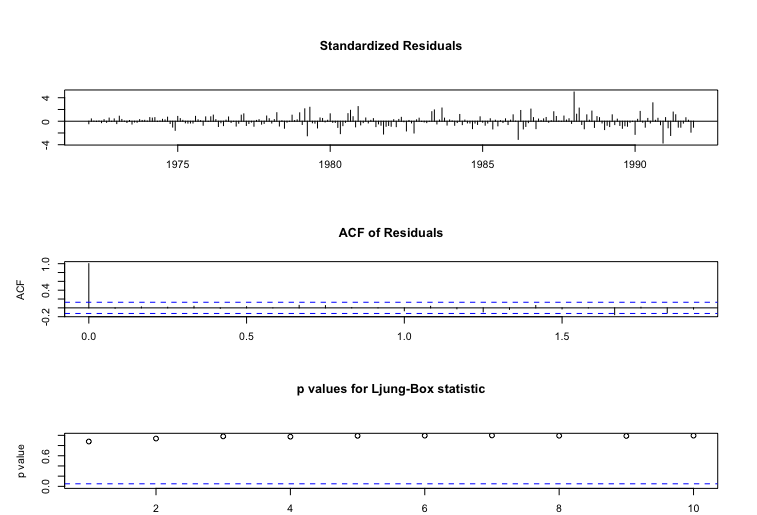
\includegraphics[width=\linewidth]{Images/P3/TSDiag_Chemicals.png}
    \caption[Residual diagnostics for the the ARIMA fit over the detrended Chemicals data.]{Residual diagnostics for the ARIMA fit over the detrended Chemicals data. These show that the residuals closely follow a normal distribution. Also, we observe that the AIC and BIC values have significantly reduced as compared to the harmonic fit over the same data.}
    \label{fig:tsdiag_chem}
\end{figure}

\begin{figure}[!htb]
    \centering
    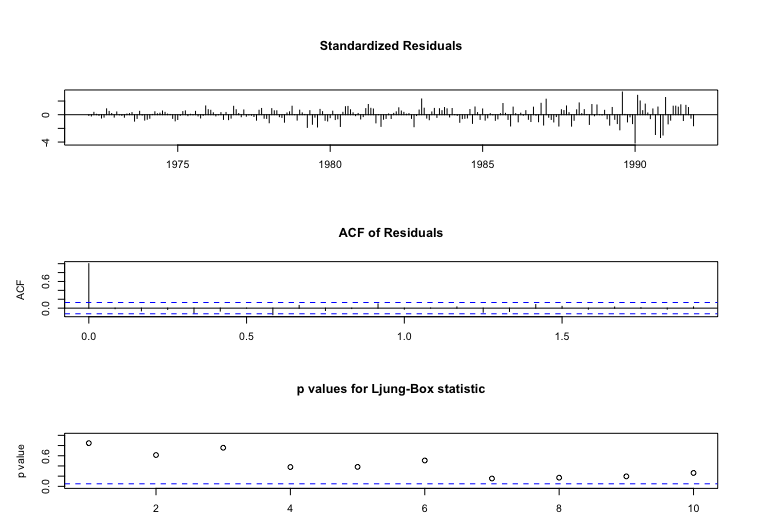
\includegraphics[width=\linewidth]{Images/P3/TSDiag_Veh.png}
    \caption[Residual diagnostics for the the ARIMA fit over the detrended Vehicles data.]{Residual diagnostics for the ARIMA fit over the detrended Vehicles data. These show that the residuals do not closely follow a normal distribution. But, we observe that the AIC and BIC values have significantly reduced as compared to the harmonic fit over the same data.}
    \label{fig:tsdiag_veh}
\end{figure}

Like before, we carry out the normality tests which align with our graphically interpreted results.
\small\begin{block}
Detrended Chemicals Data

Shapiro-Wilk normality test
W = 0.95342, p-value = 5.817e-07

Exact runs test
Runs = 121, p-value = 0.8969
alternative hypothesis: two.sided

Detrended Vehicles Data

Shapiro-Wilk normality test
W = 0.97736, p-value = 0.0007176

Exact runs test
Runs = 109, p-value = 0.1537
alternative hypothesis: two.sided
\end{block}
\normalsize Once these analyses are done, we apply BoxCox transformation (automatically chosen $\lambda_C \approx 0.19$ and $\lambda_V \approx -0.03$ for Chemicals and Vehicles data respectively) to the original data. We also do the same for the detrended data but in that case we first apply the transformation and then detrend.

The model details of the harmonic fit over the transformed data are given below.
\small\begin{block}
Transformed Chemicals Data

Call:
lm(formula = chemicals.bc.tr ~ (har + time(chemicals.bc.tr)))

Residuals:
     Min       1Q   Median       3Q      Max 
-0.40239 -0.13766 -0.00284  0.12268  0.47168 

Coefficients:
                        Estimate Std. Error t value Pr(>|t|)    
(Intercept)           -2.587e+02  3.716e+00 -69.611  < 2e-16 ***
harcos(2*pi*t)        -1.439e-02  1.607e-02  -0.895    0.371    
harsin(2*pi*t)         6.795e-02  1.608e-02   4.226 3.34e-05 ***
time(chemicals.bc.tr)  1.322e-01  1.875e-03  70.490  < 2e-16 ***
---
Signif. codes:  0 ‘***’ 0.001 ‘**’ 0.01 ‘*’ 0.05 ‘.’ 0.1 ‘ ’ 1

Residual standard error: 0.1803 on 248 degrees of freedom
Multiple R-squared:  0.9525,	Adjusted R-squared:  0.9519 
F-statistic:  1658 on 3 and 248 DF,  p-value: < 2.2e-16

Transformed Vehicles Data
Call:
lm(formula = vehicles.bc.tr ~ (har + time(vehicles.bc.tr)))

Residuals:
     Min       1Q   Median       3Q      Max 
-0.51612 -0.12429  0.02448  0.12732  0.41170 

Coefficients:
                       Estimate Std. Error t value Pr(>|t|)    
(Intercept)          -1.272e+02  3.673e+00 -34.628   <2e-16 ***
harcos(2*pi*t)        2.391e-02  1.588e-02   1.506   0.1334    
harsin(2*pi*t)        4.306e-02  1.589e-02   2.710   0.0072 ** 
time(vehicles.bc.tr)  6.534e-02  1.854e-03  35.250   <2e-16 ***
---
Signif. codes:  0 ‘***’ 0.001 ‘**’ 0.01 ‘*’ 0.05 ‘.’ 0.1 ‘ ’ 1

Residual standard error: 0.1783 on 248 degrees of freedom
Multiple R-squared:  0.834,	Adjusted R-squared:  0.832 
F-statistic: 415.3 on 3 and 248 DF,  p-value: < 2.2e-16
\end{block}
\normalsize
\begin{figure}[!htb]
    \centering
    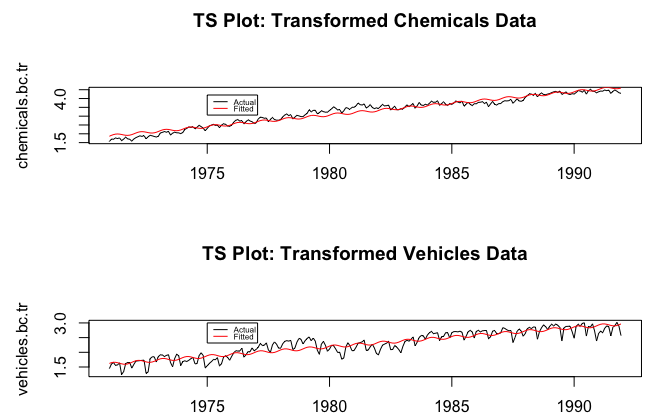
\includegraphics[width=\linewidth]{Images/P3/Lfit_BoxCox.png}
    \caption[Fitting a harmonic model with linear trend over the transformed data.]{Fitting a harmonic model with linear trend over the transformed data. There is not much improvement in the fit as compared to Fig \ref{fig:harmonic_fit}. In fact, the fit over the Chemicals data is worse. Therefore, we do not perform any other diagnostics for this model and carry on with the detrended and stabilized datasets.}
    \label{fig:harmonic_bc_fit}
\end{figure}

Here, in Fig \ref{fig:diff_bc_plots} we observe the temporal patterns of the stabilized datasets (transformed, detrended, and seasonality removed).
\begin{figure}[!htb]
    \centering
    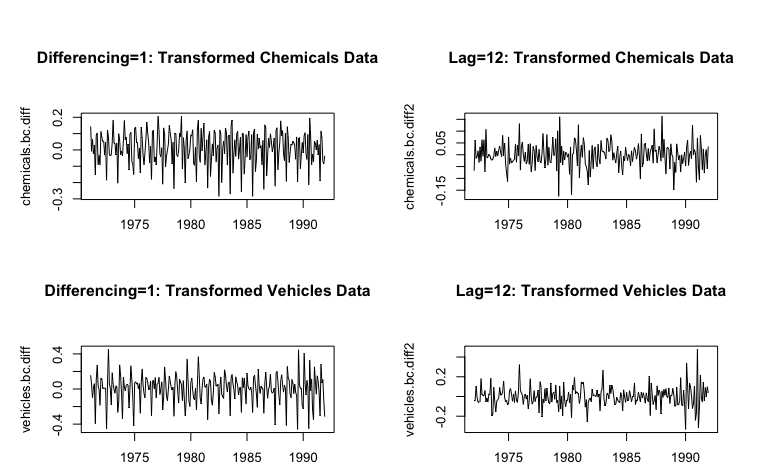
\includegraphics[width=\linewidth]{Images/P3/Diff_BC_Plots.png}
    \caption[Time series plots of the stabilized data.]{Time series plots of the stabilized data. The plots are constructed the same way as in Fig \ref{fig:diff_plots}. However, we see that the stabilized data appears to be more stationary than before.}
    \label{fig:diff_bc_plots}
\end{figure}

Now, we check the different ACF plots depicted in Fig \ref{fig:acf_bc_det}.
\begin{figure}[!htb]
    \centering
    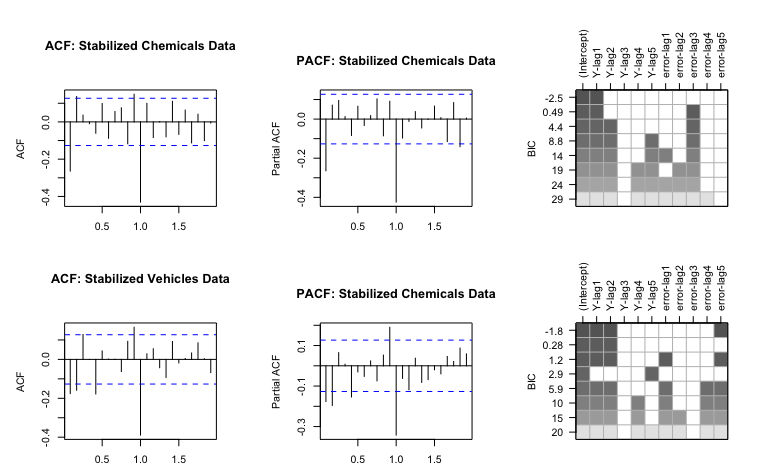
\includegraphics[width=\linewidth]{Images/P3/ACFs_BC_Plots.png}
    \caption[ACF, PACF, and ARMA subset plots for the stabilized Chemicals and Vehicles data.]{ACF, PACF, and ARMA subset plots for the stabilized Chemicals and Vehicles data. These show that the detrended data could possible have both AR and MA parts like before but the AIC and BIC values could be significantly reduced (since $\lambda_C \approx 0.19$ and $\lambda_V \approx -0.03$ for Chemicals and Vehicles data respectively) as compared to Fig \ref{fig:acf_det}.}
    \label{fig:acf_bc_det}
\end{figure}
The EACF matrices for these stabilized datasets are given here.
\small\begin{block}
> eacf(chemicals.bc.diff2)
AR/MA
  0 1 2 3 4 5 6 7 8 9 10 11 12 13
0 x x o o o o o o o o x  x  o  o 
1 x x o o o o o o o o o  x  x  o 
2 x x o o o o o o o o o  x  x  o 
3 o x x o o o o o o o o  x  x  o 
4 x x o o o o o o o o o  x  x  x 
5 x x o o o o o o o o o  x  o  x 
6 x o o o x o o o o o o  x  o  o 
7 x o o x o o o o o o o  x  x  o

> eacf(vehicles.bc.diff2)
AR/MA
  0 1 2 3 4 5 6 7 8 9 10 11 12 13
0 x x o o x o o o o o x  x  o  o 
1 x x o o x o o o o o o  x  x  o 
2 x o o o x o o o o o o  x  x  x 
3 o o x o x o o o o o o  x  x  x 
4 o x x x o o o o o o o  x  x  o 
5 x x x x o o o o o o o  x  x  o 
6 x x o x o o o o o o o  x  x  o 
7 x x o o o o x o o o o  x  o  o 
\end{block}
\normalsize As expected from Fig \ref{fig:acf_bc_det}, we have greatly reduced the AIC and BIC values using transformation. The model details obtained using the auto.arima function are given here. It is noteworthy that, while the number of parameters for the Chemicals data remain the same as before, we have been able to reduce one parameter in case of the Vehicles data. Hence, we do not further check the residuals.
\small\begin{block}
> chemicals.bc.diff2.arima = auto.arima(chemicals.bc.diff2)
> chemicals.bc.diff2.arima

Series: chemicals.bc.diff2 
ARIMA(2,0,2)(0,0,1)[12] with zero mean 

Coefficients:
          ar1      ar2     ma1     ma2     sma1
      -0.9330  -0.9102  0.7469  0.7854  -0.6996
s.e.   0.0548   0.0595  0.0850  0.0741   0.0641

sigma^2 estimated as 0.001787:  log likelihood=415.93
AIC=-819.86   AICc=-819.5   BIC=-799.01

> vehicles.bc.diff2.arima = auto.arima(vehicles.bc.diff2)
> vehicles.bc.diff2.arima

Series: vehicles.bc.diff2 
ARIMA(0,0,2)(0,0,2)[12] with zero mean 

Coefficients:
          ma1      ma2     sma1     sma2
      -0.2106  -0.1494  -0.6332  -0.1205
s.e.   0.0676   0.0740   0.0678   0.0723

sigma^2 estimated as 0.006902:  log likelihood=252.91
AIC=-495.82   AICc=-495.56   BIC=-478.44
\end{block}

\normalsize Therefore, from the above results, it can be concluded that transformation improves the fit of these models. In order to check the cross-correlation between the Chemicals and Vehicles data, we use the ccf function in R (Fig \ref{fig:ccf}). This shows that the sales of chemicals and vehicles are positively correlated. 

\begin{figure}[!htb]
    \centering
    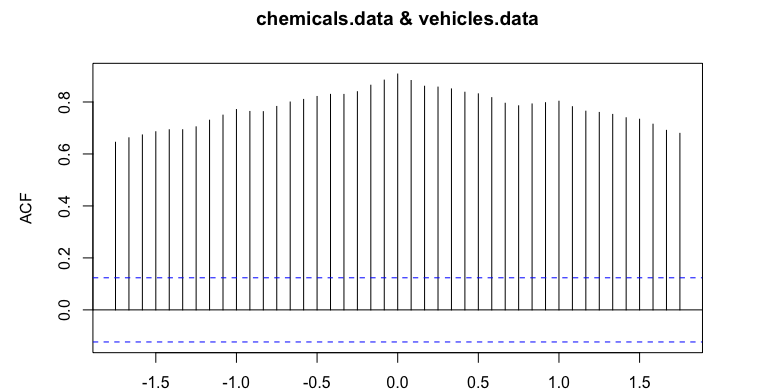
\includegraphics[width=\linewidth]{Images/P3/CCF.png}
    \caption[Cross-correlation plot of Chemicals and Vehicles data.]{Cross-correlation plot of Chemicals and Vehicles data.}
    \label{fig:ccf}
\end{figure}

\item The strong positive correlation between the Chemicals and Vehicles data could be attributed to the increase of vehicle usage over time thereby necessitating more use of chemicals not only for vehicle parts but also for additional utilities like stain removers etc. However, if the month-to-month variation is considered, there are bigger variations in the sales of vehicles. This is because Chemical sales on a monthly basis will not fluctuate much as chemicals are required in a variety of industries. But in case of vehicles, there are additional factors involved such as the economic slowdown which significantly affect the sales.

\end{enumerate}

\section{Problem 4}
%\addcontentsline{toc}{section}{Problem 4}
France has enjoyed a long and storied history as a world leader in culture, food,
literature, film, and revolutions. Over its history, the average life expectancy of people in France
has changed notably. The time series object described below contains the annual average life
expectancy in France (measured in years lived), measured during the years 1816 to 2019. The
data is in the file FLE.txt. \\

\noindent Analyze the data in the time series and write a report addressing the following:

\begin{enumerate}[label=(\alph*)]
    \item What trend model(s) best capture the trends in French life expectancy over time?
    \item Are there any noticeable patterns, or observations apparent in the series? Can you tell from
your plot what could be the causes of your observations?
    \item Regardless of what you observe, suppose you apply some transformation to the data, how
does the new data looks like? Any changes in trend?
    \item For the various models you tried, assess the fit of the models using any tools at your disposal. Perform any necessary test to make sure sure your model is appropriate. Write down the equation of your final model. Are any transformations of the data necessary? Perform all diagnostics tests.
\end{enumerate}

\noindent Now conclude with brief summary: How the life expectancy changes over time, both long-term
over the observed period of years, and in terms of patterns of year-to-year variation. Add any
necessary graphs, tests and/or confidence interval etc...

\subsection{R Code}
\lstinputlisting[language=R]{Codes/Midterm_2_P4.R}
\subsection{Results}
\begin{enumerate}[label=(\alph*)]
    \item \begin{minipage}[!h]{\linewidth}
        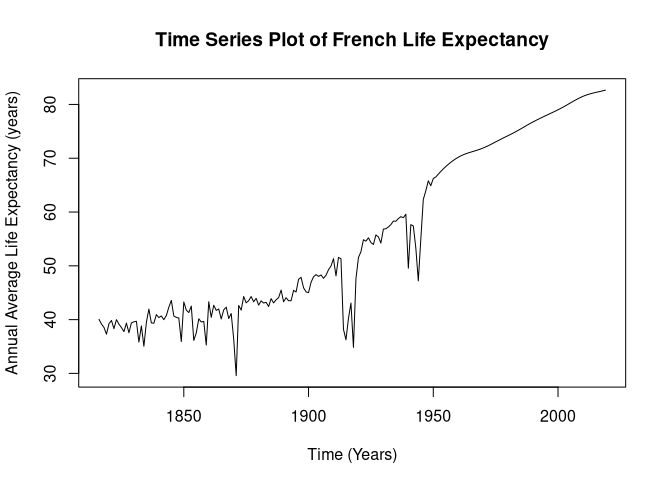
\includegraphics[width=0.9\linewidth]{Images/P4/FLE_Plot.png}
        \captionof{figure}{Time series plot of the French life expectancy data.}
        \label{fig:fle_plot}
    \end{minipage}

From Fig \ref{fig:fle_plot} it can be said that a quadratic trend is suitable for this dataset. The model summary is shown here.
\small\begin{block}
Call:
lm(formula = fle.data ~ time(fle.data) + I(time(fle.data)^2))

Residuals:
     Min       1Q   Median       3Q      Max 
-17.2140  -1.3665   0.4999   1.8464   5.6716 

Coefficients:
                      Estimate Std. Error t value Pr(>|t|)    
(Intercept)          3.499e+03  3.042e+02   11.50   <2e-16 ***
time(fle.data)      -3.849e+00  3.175e-01  -12.12   <2e-16 ***
I(time(fle.data)^2)  1.069e-03  8.279e-05   12.92   <2e-16 ***
---
Signif. codes:  0 ‘***’ 0.001 ‘**’ 0.01 ‘*’ 0.05 ‘.’ 0.1 ‘ ’ 1

Residual standard error: 3.668 on 201 degrees of freedom
Multiple R-squared:  0.946,	Adjusted R-squared:  0.9455 
F-statistic:  1762 on 2 and 201 DF,  p-value: < 2.2e-16
\end{block}
\normalsize Here, we observe that the F-statistic and the residual standard are quite high. Moreover, the augmented Dickey-Fuller stationarity test (Dickey-Fuller = -2.9107, Lag order = 5, p-value = 0.1945) confirms that the original data is not stationary. However, by only visually observing the original data (Fig \ref{fig:fle_plot}), we can say that the quadratic fit (Fig \ref{fig:qfit_fle}) is the best trend for this dataset.
\begin{figure}[!htb]
    \centering
    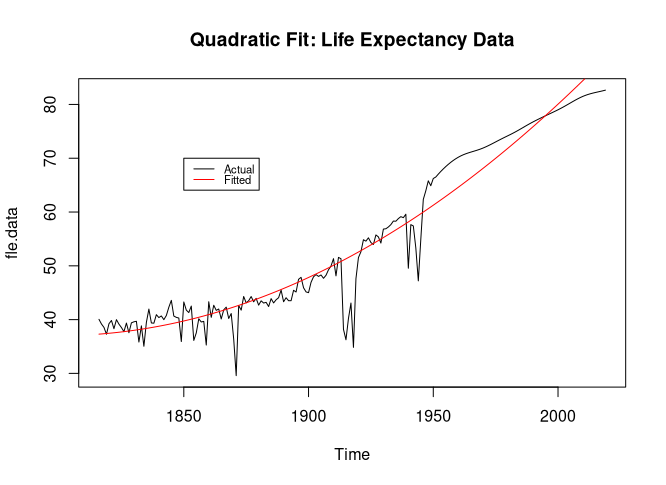
\includegraphics[width=0.9\linewidth]{Images/P4/QFit_FLE.png}
    \caption[Quadratic fit over the original French life expectancy data.]{Quadratic fit over the original French life expectancy data. The fit performs poorly from 1950 onward as we observe a linear trend from 1950-2019.}
    \label{fig:qfit_fle}
\end{figure}
\item The fluctuations in the dataset are mostly present before 1950. The increase in the life expectancy values between 1816-1850 could be attributed to the advancements in medicine. However, the sharp drops in the values, particularly during mid 1915-1920 and mid 1940s could be caused by the two world wars. Interestingly, the life expectancy increases post 1950 which could be primarily attributed to the invention of modern healthcare and economic growth.
\item \begin{minipage}[!h]{\linewidth}
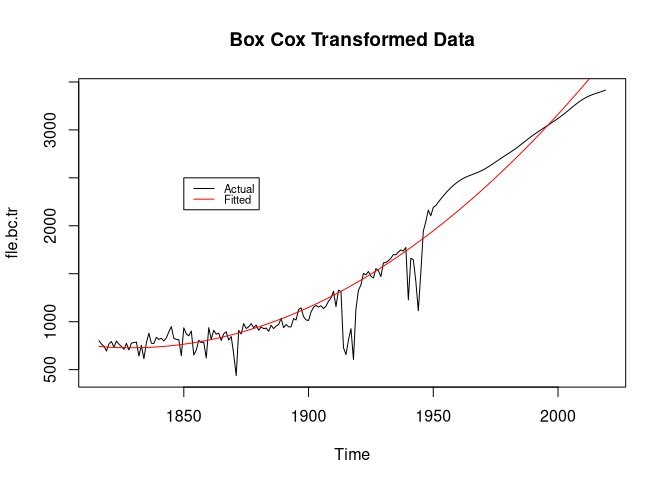
\includegraphics[width=\linewidth]{Images/P4/FLE_BC.png}
\captionof{figure}[Transformed FLE Data using Box Cox method.]{Transformed FLE Data using Box Cox method. Here, this transformation is obtained by auto-setting $\lambda \approx 1.99$. The quadratic trend still remains.}
\label{fig:qfit_bc_fle}
\end{minipage}

The model fit summary for this transformed dataset is given here.
\small\begin{block}
Call:
lm(formula = fle.bc.tr ~ time(fle.bc.tr) + I(time(fle.bc.tr)^2))

Residuals:
    Min      1Q  Median      3Q     Max 
-782.46  -70.39   23.94   83.28  305.68 

Coefficients:
                       Estimate Std. Error t value Pr(>|t|)    
(Intercept)           2.787e+05  1.494e+04   18.66   <2e-16 ***
time(fle.bc.tr)      -3.040e+02  1.559e+01  -19.50   <2e-16 ***
I(time(fle.bc.tr)^2)  8.311e-02  4.064e-03   20.45   <2e-16 ***
---
Signif. codes:  0 ‘***’ 0.001 ‘**’ 0.01 ‘*’ 0.05 ‘.’ 0.1 ‘ ’ 1

Residual standard error: 180.1 on 201 degrees of freedom
Multiple R-squared:  0.9625,	Adjusted R-squared:  0.9621 
F-statistic:  2579 on 2 and 201 DF,  p-value: < 2.2e-16
\end{block}
\normalsize
\item The residual diagnostics for the quadratic model are shown in Fig \ref{fig:res_qfit_fle}.
\begin{figure}[!htb]
    \centering
    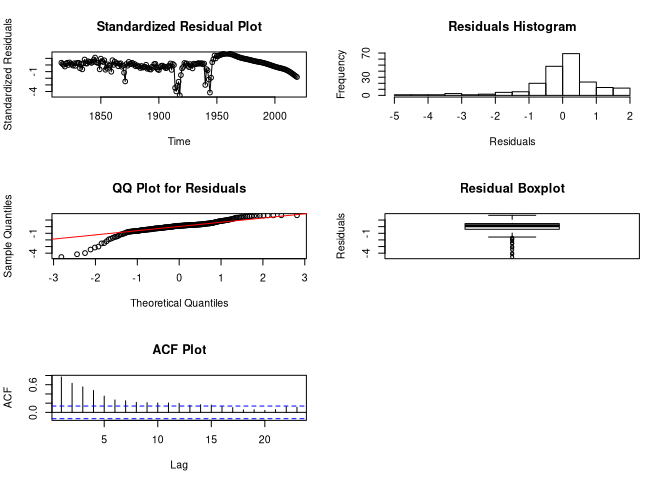
\includegraphics[width=\linewidth]{Images/P4/Residual_QFit.png}
    \caption[Residual diagnostics for the quadratic model.]{Residual diagnostics for the quadratic model. Here, we observe that this model fits poorly as the residuals follow a non-normal distribution.}
    \label{fig:res_qfit_fle}
\end{figure}
We further verify the non-normality of the residuals using the Shapiro-Wilk and Exact Runs tests.
\small\begin{block}
Quadratic Model

Shapiro-Wilk normality test
W = 0.88032, p-value = 1.21e-11

Exact runs test
Runs = 46, p-value = 3.374e-16
alternative hypothesis: two.sided
\end{block}
\normalsize Next, we detrend the transformed dataset (Fig \ref{fig:detrend_fle}) using two differences because of the quadratic trend (i.e. the transformed dataset is not stationary). Since no seasonality is present, we set lag=1.
\begin{figure}[!htb]
    \centering
    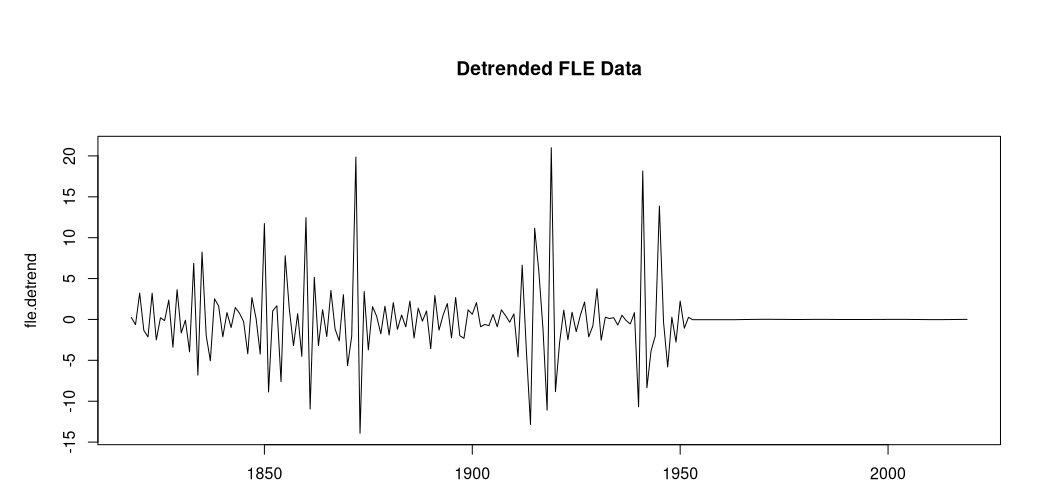
\includegraphics[width=\linewidth]{Images/P4/Detrend_FLE.png}
    \caption[Plot of the detrended FLE data.]{Plot of the detrended FLE data. This shows that we have achieved stationarity and can now proceed with various ARIMA modeling. We also verify this using the augmented Dickey-Fuller test (Dickey-Fuller = -10.009, Lag order = 5, p-value = 0.01) where we accept the alternative hypothesis of stationarity.}
    \label{fig:detrend_fle}
\end{figure}
Once the detrending is done, we check the ACF, PACF, EACF, and the ARMA subset plots as given in Fig. \ref{fig:acf_fle}.

\begin{figure}[!htb]
    \centering
    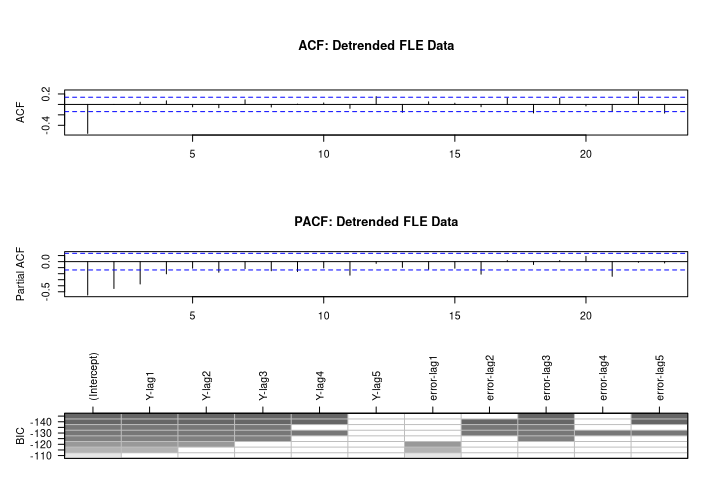
\includegraphics[width=\linewidth]{Images/P4/ACF_Plots_FLE.png}
    \caption[ACF, PACF, and ARMA subset plots of the detrended FLE data]{ACF, PACF, and ARMA subset plots of the detrended FLE data. From these we can say that ARMA(p, q) is a suitable model.}
    \label{fig:acf_fle}
\end{figure}
\small\begin{block}
> eacf(fle.detrend)

AR/MA
  0 1 2 3 4 5 6 7 8 9 10 11 12 13
0 x o o o o o o o o o o  x  x  o 
1 x o o o o o o o o o o  o  o  o 
2 x x o o o o o o o o o  o  o  o 
3 x o x o o o o o o o o  o  o  o 
4 x o x x x o o o o o o  o  o  o 
5 x x o o x o o o o o o  o  o  o 
6 x x x o o o x o o o o  o  o  o 
7 x x x o o o o x o o o  o  o  o
\end{block}
\normalsize Initially, we consider ARMA(1, 1) model or ARIMA(1, 0, 1). The model fit summary is given here.
\small\begin{block}
>arima(x = fle.detrend, order = c(1, 0, 1))

Coefficients:
          ar1     ma1  intercept
      -0.2498  -1.000     0.0017
s.e.   0.0680   0.013     0.0025

sigma^2 estimated as 6.765:  log likelihood = -482.63,  aic = 971.26
\end{block}
\normalsize We also perform the residual diagnostics (Figures \ref{fig:tsdiag_fle_arma_11} and \ref{fig:res_fle_arma_11})and apply the normality checks.
\begin{figure}[!htb]
    \centering
    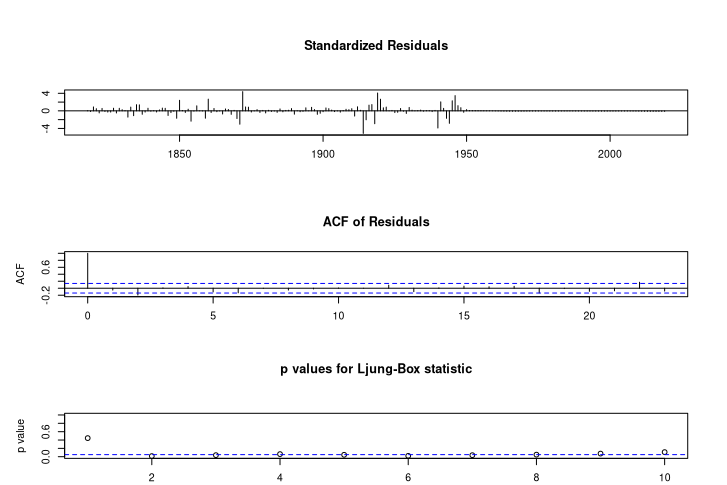
\includegraphics[width=\linewidth]{Images/P4/TSDiag_ARMA_11.png}
    \caption[Residual diagnostics for the ARMA(1, 1) model for the FLE data.]{Residual diagnostics for the ARMA(1, 1) model for the FLE data.}
    \label{fig:tsdiag_fle_arma_11}
\end{figure}
\begin{figure}[!htb]
    \centering
    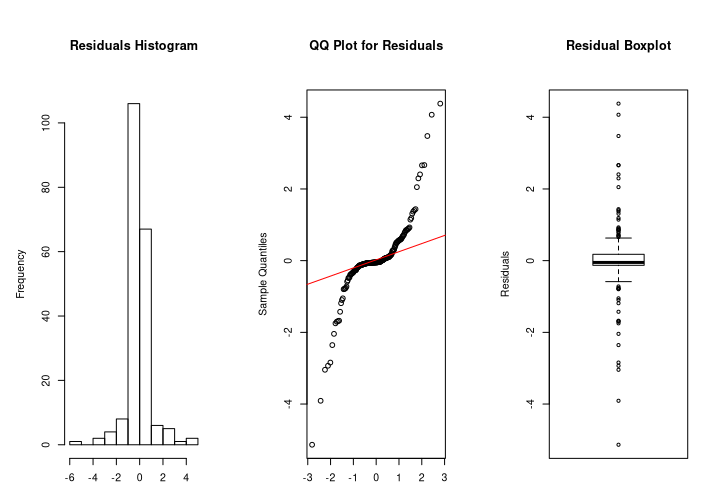
\includegraphics[width=\linewidth]{Images/P4/Residuals_FLE_ARMA_11.png}
    \caption[Residual plots for the ARMA(1, 1) model for the FLE data.]{Residual plots for the ARMA(1, 1) model for the FLE data.}
    \label{fig:res_fle_arma_11}
\end{figure}
The residual diagnostics show that the ARMA(1, 1) residuals do not closely follow a normal distribution. This is further confirmed by the Shapiro-Wilk and Runs tests.
\small\begin{block}
ARMA(1, 1) for the detrended FLE data

Shapiro-Wilk normality test
W = 0.76725, p-value < 2.2e-16

Exact runs test
Runs = 86, p-value = 0.02855
alternative hypothesis: two.sided

> AIC(model)
[1] 973.2626
> BIC(model)
[1] 986.4957
\end{block}
\normalsize Next, we try with ARMA(1, 2) to see if we have a better fit.
\small\begin{block}
Call:
arima(x = fle.detrend, order = c(1, 0, 2))

Coefficients:
         ar1      ma1     ma2  intercept
      0.5658  -1.8831  0.8831     0.0017
s.e.  0.0946   0.0600  0.0594     0.0009

sigma^2 estimated as 6.266:  log likelihood = -476.12,  aic = 960.25
\end{block}
\normalsize The residual diagnostics (Figures \ref{fig:tsdiag_fle_arma_12} and \ref{fig:res_fle_arma_12}) and normality checks are carried out like before.
\begin{figure}[!htb]
    \centering
    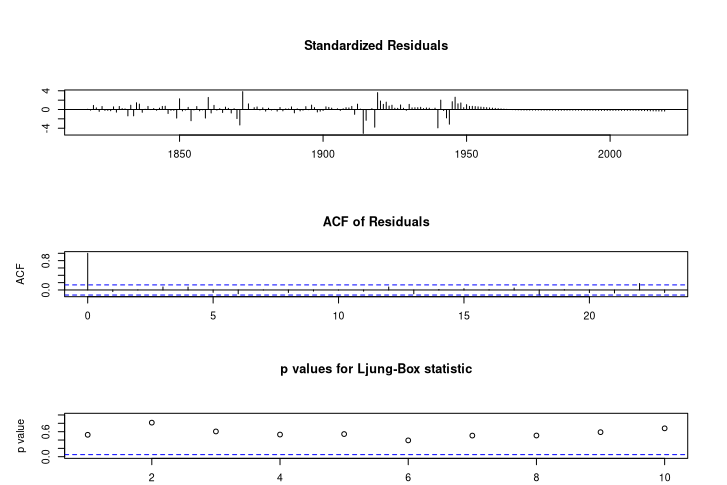
\includegraphics[width=\linewidth]{Images/P4/TSDiag_FLE_ARMA_12.png}
    \caption[Residual diagnostics for the ARMA(1, 2) model for the FLE data.]{Residual diagnostics for the ARMA(1, 2) model for the FLE data.}
    \label{fig:tsdiag_fle_arma_12}
\end{figure}
\begin{figure}[!htb]
    \centering
    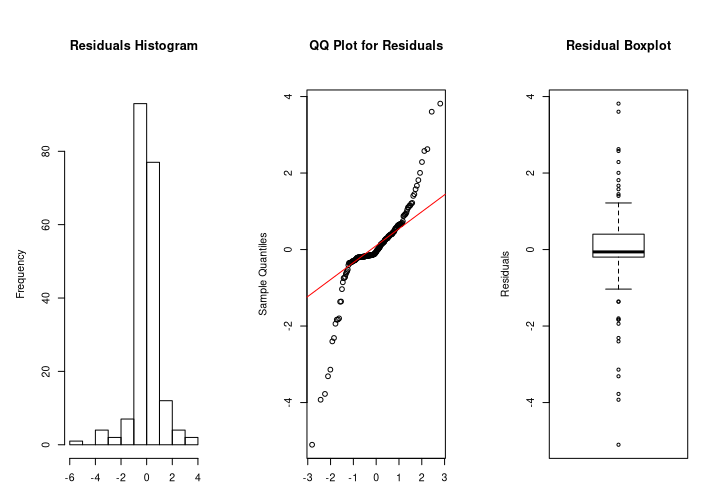
\includegraphics[width=\linewidth]{Images/P4/Residuals_FLE_ARMA_12.png}
    \caption[Residual plots for the ARMA(1, 2) model for the FLE data.]{Residual plots for the ARMA(1, 2) model for the FLE data.}
    \label{fig:res_fle_arma_12}
\end{figure}
The residual diagnostics show that the ARMA(1, 1) residuals do not closely follow a normal distribution. This is further confirmed by the Shapiro-Wilk and Runs tests.
\small\begin{block}
ARMA(1, 2) for the detrended FLE data

Shapiro-Wilk normality test
W = 0.81151, p-value = 6.773e-15

Exact runs test
Runs = 66, p-value = 4.192e-07
alternative hypothesis: two.sided

> AIC(model)
[1] 962.246
> BIC(model)
[1] 978.7874
\end{block}
\normalsize From these we can conclude that ARMA(1, 1) is preferred model. However, to obtain a better fit, we use the auto.arima function and check the effect of transformation. The model summary including the AIC and BIC values and the confidence intervals of the parameters are given here.
\small\begin{block}
> fle.auto.arima = auto.arima(fle.detrend)
> fle.auto.arima
Series: fle.detrend 
ARIMA(1,0,3) with zero mean 

Coefficients:
         ar1      ma1     ma2      ma3
      0.7382  -2.0855  1.2361  -0.1467
s.e.  0.0960   0.1212  0.2218   0.1026

sigma^2 estimated as 6.436:  log likelihood=-475.51
AIC=961.01   AICc=961.32   BIC=977.55

> fle.bc.auto.arima = auto.arima(fle.detrend, lambda="auto")
> fle.bc.auto.arima
Series: fle.detrend 
ARIMA(1,0,2) with non-zero mean 
Box Cox transformation: lambda= 0.7566293 

Coefficients:
         ar1      ma1     ma2     mean
      0.5021  -1.6531  0.7389  -1.3864
s.e.  0.2453   0.1990  0.1701   0.0253

sigma^2 estimated as 4.409:  log likelihood=-435.52
AIC=881.04   AICc=881.34   BIC=897.58

> confint(fle.bc.auto.arima)
                2.5 %     97.5 %
ar1        0.02135014  0.9827585
ma1       -2.04318152 -1.2630966
ma2        0.40548839  1.0722244
intercept -1.43600896 -1.3367935
\end{block}
\normalsize Here, we see that the transformed dataset has lower AIC and BIC values along with lesser parameters wherein the confidence intervals do not contain zero. Therefore, data transformation is required.

So from the above analyses, the final model chosen is the ARIMA(1, 2, 2) model (ARMA(1, 2) for the second order differences) where BoxCox transformation ($\lambda \approx 0.75$) is used. The model equation is given by Eq. \eqref{eq:final_model}.
\begin{equation}
    Z_t = -1.3864 + 0.5021Z_{t-1} + 1.6531\varepsilon_{t-1} -0.7389\varepsilon_{t-2} + \varepsilon_t
    \label{eq:final_model}
\end{equation}
 where $\varepsilon \sim \mathcal{N}(0, 4.409)$ and $Z_t = $ BoxCox($\nabla^2{X_t}$, $\lambda$), $\lambda \approx 0.75$, $t = \{1, 2, 3, \dots\}$, and $X_t$ being the original FLE data.
\end{enumerate}

\noindent If the entire duration of the time series is considered, then the life expectancy has greatly varied before 1950 but there is an overall increase in the life expectancy. From 1950 onward, the life expectancy keeps on increasing linearly. 

\noindent When individual years are taken into account, then the sharp increments and decrements in the values can be attributed to the improved healthcare systems and degrading economy or wars respectively.


%\appendix
%\section{Appendix}
%\input{Chapters/06_Appendix1}


%---------------------------------------------------------------------------------
%	Example SECTION (Remove this section to finalize the report.


%\section{Example steps}
%% These are some example steps 
% Refer https://www.overleaf.com/learn/how-to/Creating_a_document_in_Overleaf


\subsection{Sub Sections}

Use section and subsection commands to organize your document. \LaTeX{} handles all the formatting and numbering automatically. Use ref and label commands for cross-references.

\subsection{Comments}

Comments can be added to the margins of the document using the \todo{Here's a comment in the margin!} todo command, as shown in the example on the right. You can also add inline comments too:

\todo[inline, color=green!40]{This is an inline comment.}

\subsection{Tables and Figures}

Use the table and tabular commands for basic tables --- see Table~ \ref{tab:widgets}, for example. You can upload a figure (JPEG, PNG or PDF) using the files menu. To include it in your document, use the include graphics command as in the code for Figure~\ref{fig:Speed vs. Torque from Pittman} below.

\begin{table}[h]
\centering
\begin{tabular}{|l|r|}
\hline
Item & Quantity \\\hline
Widgets & 42 \\ \hline
Gadgets & 13 \\ \hline
\end{tabular}
\caption{\label{tab:widgets}An example table.}
\end{table}

% Commands to include a figure:
\begin{figure}[hbt!]
    \centering
    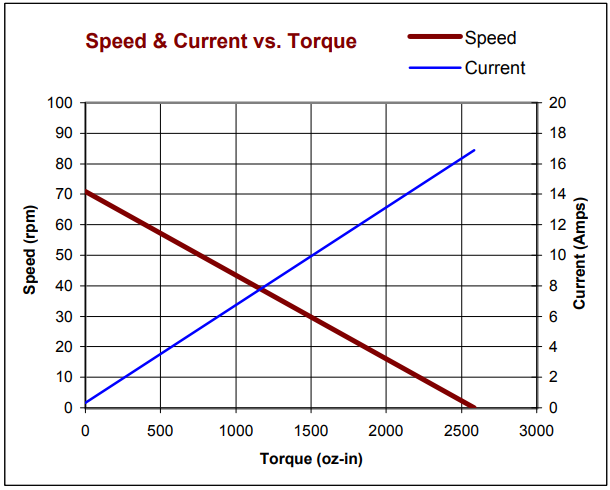
\includegraphics[width=0.9\textwidth]{Images/SpeedvsTorque.png}
    \caption{Speed vs. Torque from Pittman motor data sheet}
    \label{fig:Speed vs. Torque from Pittman}
\end{figure}





\subsection{Mathematics}

\LaTeX{} is great at typesetting mathematics. Let $X_1, X_2, \ldots, X_n$ be a sequence of independent and identically distributed random variables with $\text{E}[X_i] = \mu$ and $\text{Var}[X_i] = \sigma^2 < \infty$, and let
$$S_n = \frac{X_1 + X_2 + \cdots + X_n}{n}
      = \frac{1}{n}\sum_{i}^{n} X_i$$
denote their mean. Then as $n$ approaches infinity, the random variables $\sqrt{n}(S_n - \mu)$ converge in distribution to a normal $\mathcal{N}(0, \sigma^2)$.

\subsection{Lists}

You can make lists with automatic numbering \dots

\begin{enumerate}
\item Like this,
\item and like this.
\end{enumerate}
\dots or bullet points \dots
\begin{itemize}
\item Like this,
\item and like this.
\end{itemize}

%% cite an article
\subsection{Bibliography}
\begin{itemize}
    \item Adding bibliography to document
Some claim \cite{gratzer2007more}.
\end{itemize}

\subsection{Hyperlink to a website}
%% Hyperlink to a website
\begin{itemize}
    \item \href{https://www.overleaf.com/latex/templates/a-quick-guide-to-latex/fghqpfgnxggz}{Hyperlink to a website}.
\end{itemize}



\subsection{Learn LaTeX in 30 minutes}
\begin{itemize}
    \item \href{https://www.overleaf.com/learn/latex/Learn_LaTeX_in_30_minutes}{Link to overleaf website}.
\end{itemize}

 % Remove this line to finalize the report.
%---------------------------------------------------------------------------------


\end{document}


% Note: Again, you don’t need to answer just the above questions. They are being provided to give you a flavor of what is required for each section. Use your judgment and initiative to add or subtract based on the specific homework. You can add any other conclusion or discuss any other aspect of your effort that you think it is important to highlight.

% Also ensure to attach the MATLAB or MULTISIM files with this report